\documentclass{article}

\usepackage{graphicx} % Required for inserting images
\usepackage{amsmath} % For math equations if needed
\usepackage{url}     % For formatting URLs
\usepackage{booktabs} % For better table lines
\usepackage{caption}  % For captions
\usepackage[utf8]{inputenc}
\usepackage[T1]{fontenc}
\usepackage{float} % Added for stronger figure placement control [H]
\usepackage{siunitx} % For aligning numbers in tables
\usepackage{subcaption} % For subfigures
\usepackage[margin=1in]{geometry} % Set 1-inch margins
\usepackage{times} % Use Times New Roman font
\usepackage{helvet} % Use Helvetica for sans-serif
\usepackage{courier} % Use Courier for monospace
\usepackage{hyperref} % For clickable links, refs, and metadata

\hypersetup{
    pdfauthor={Abhilash Chadhar, Kartik Chadhar},
    pdftitle={AdaptiVision: Scene-Adaptive Confidence Thresholding for Object Detection - Performance Analysis on COCO},
    pdfsubject={Computer Vision, Object Detection},
    pdfkeywords={Object Detection, YOLOv8, Adaptive Thresholding, Scene Complexity, COCO, Computer Vision},
    colorlinks=true, % false: boxed links; true: colored links
    linkcolor=blue,  % color of internal links (sections, figures, etc.)
    citecolor=blue,  % color of links to bibliography
    filecolor=magenta, % color of file links
    urlcolor=blue    % color of external links
}

% --- Paper Title ---
\title{AdaptiVision: Scene-Adaptive Confidence Thresholding for Object Detection - Performance Analysis on COCO}

% --- Author Info (Standard Style) ---
\author{
  Abhilash Chadhar \\
  Axelera AI / Indian Institute of Space Science and Technology \\
  \\
  \texttt{abhilashchadhar@gmail.com} \\
  \and \\
  Kartik Chadhar \\
  All India Institute of Medical Sciences (AIIMS), Delhi \\
  \\
  \texttt{kartikchadhar@gmail.com}
}

\date{\today} % Or specify a date

\pagestyle{empty} % Remove page numbers for arXiv

\begin{document}

\maketitle

% --- Abstract --- revised significantly
\begin{abstract}
Fixed confidence thresholds in object detection models limit robustness across diverse visual scenes. This paper investigates AdaptiVision, a post-processing technique designed to enhance detection by dynamically adjusting the confidence threshold for a YOLOv8n model based on scene complexity heuristics (object count, size variance, density) derived from initial low-confidence detections. Optional rule-based context awareness and class-specific biases can further modulate the threshold. We perform a rigorous evaluation on the COCO 2017 validation dataset (5000 images) using standard mAP metrics. The results show that while AdaptiVision increases the average number of detected objects per image (6.43 vs. 4.95) and improves average processing speed by nearly 1.5x compared to the standard fixed-threshold approach (0.024s vs. 0.034s on test hardware), it leads to a decrease in overall detection accuracy (mAP@[.50:.95]: 0.340 vs. 0.355 baseline; AR@[.50:.95]: 0.428 vs. 0.464 baseline). This performance degradation, despite identifying more objects faster, highlights the limitations of the current heuristic approach in effectively balancing precision and recall according to standard COCO metrics. The study underscores the challenge of designing adaptive heuristics that generalize well and the importance of comprehensive evaluation beyond simple object counts or speed metrics.
\end{abstract}

% --- Introduction --- revised slightly
\section{Introduction}

Object detection—the task of identifying and localizing objects within an image—is a cornerstone of modern computer vision, enabling applications such as autonomous driving, robotics, surveillance, and image retrieval. State-of-the-art detectors, particularly those based on deep learning like the YOLO family \cite{YOLOv3, YOLOv4, YOLOv6, YOLOv7}, typically assign a confidence score to each potential detection. Filtering these potential detections using a confidence threshold is crucial.

The common practice involves setting a single, fixed confidence threshold. While straightforward, this approach faces limitations: a threshold optimized for simple scenes might miss detections in complex ones (low recall), while a lower threshold increases false positives in simple scenes (low precision). This inflexibility motivates research into adaptive methods.

We analyze AdaptiVision, a post-processing methodology attempting to adapt the confidence threshold based on scene characteristics estimated directly from initial YOLOv8n \cite{YOLOv8} detection results using heuristics (object count, size variance, density). AdaptiVision operates as a lightweight layer applied after initial inference.

This paper presents a rigorous evaluation using standard COCO mAP metrics on the full COCO 2017 validation dataset (val2017, 5000 images) \cite{COCO}. The core contributions are:
\begin{enumerate}
    \item Analysis of a heuristic method for estimating scene complexity from initial detections.
    \item Evaluation of a dynamic threshold mapping mechanism based on this complexity.
    \item Assessment of optional rule-based context and class biases integration.
    \item An experimental evaluation on COCO val2017 using standard mAP metrics, comparing AdaptiVision to a baseline.
    \item An analysis of the trade-offs observed between object counts, processing speed, and standard accuracy metrics (mAP, AR).
\end{enumerate}

This paper is structured as follows: Section \ref{sec:related} discusses related work. Section \ref{sec:methodology} details the AdaptiVision methodology. Section \ref{sec:experiments} outlines the experimental setup and results on COCO val2017. Section \ref{sec:discussion} discusses the implications and limitations, and Section \ref{sec:conclusion} concludes the paper.

% --- Related Work ---
\section{Related Work} \label{sec:related}

The challenge of optimizing object detection performance across diverse scenes has motivated research beyond standard architectures with fixed parameters. Several avenues have been explored to make detection more adaptive and context-aware.

\paragraph{Adaptive Non-Maximum Suppression (NMS):} Standard NMS uses a fixed Intersection over Union (IoU) threshold to suppress redundant bounding boxes. Recognizing that optimal suppression might depend on object density, methods like Adaptive NMS \cite{AdaptiveNMS} propose adjusting the IoU threshold dynamically based on the density of nearby detections. Soft-NMS \cite{SoftNMS} offers an alternative by decaying the scores of overlapping boxes instead of eliminating them outright. While related to adapting parameters based on detection characteristics, these methods focus on the NMS stage, whereas AdaptiVision targets the initial confidence filtering threshold *based on broader scene complexity metrics rather than just local density for NMS*.

\paragraph{Confidence Calibration:} Some research focuses on improving the reliability of the confidence scores output by detectors, ensuring they better reflect the true probability of a correct detection \cite{Calibration}. While valuable, calibration typically aims to improve the \textit{interpretation} of existing scores rather than dynamically changing the \textit{filtering threshold} based on scene properties *in response to overall scene complexity*.

\paragraph{Context-Aware Object Detection:} Incorporating scene context can significantly improve detection accuracy. Early approaches often used graphical models or statistical co-occurrence information. More recent deep learning methods, such as Relation Networks \cite{RelationNet}, explicitly model object relationships using dedicated network modules (e.g., attention mechanisms, graph neural networks) to learn contextual dependencies. These approaches often require significant architectural changes and additional training data. AdaptiVision incorporates a simpler, optional form of context using predefined, rule-based object relationships applied during its post-processing threshold adjustment, avoiding architectural modifications *and focusing primarily on complexity-driven thresholding rather than learned contextual reasoning as the main driver*.

\paragraph{Adaptive Confidence Thresholding:} The idea of adjusting the confidence threshold itself has been explored, particularly for specific applications. Lee et al. \cite{LeeLiDARAdapt} proposed adjusting thresholds for 3D LiDAR object detection based on the object's distance from the sensor, addressing range-dependent performance variations. In the domain of multi-object tracking, Ma et al. \cite{MaByteTrackAdapt} investigated adapting the threshold distinguishing high-confidence and low-confidence detections within the ByteTrack algorithm, using insights from overall detections to potentially improve track association. AdaptiVision differs by focusing on 2D object detection filtering and using a specific combination of object count, size variance, and density from initial detections to derive a scene complexity score, which then directly modulates the filtering threshold for each image, *offering a more general scene complexity approach compared to application-specific adjustments like distance or tracking-specific thresholds*.

\paragraph{Contribution of AdaptiVision:} Compared to the related work, AdaptiVision's contribution lies in its specific heuristic approach to scene complexity estimation derived directly from initial, low-confidence detections and its use as a lightweight, post-processing module to dynamically adjust confidence thresholds. It combines complexity analysis, class-specific biases, and optional rule-based context in a unified framework that can be integrated with standard object detectors without retraining or architectural changes. This work evaluates the effectiveness of this specific heuristic approach using standard benchmarks.

% --- Methodology ---
\section{Methodology} \label{sec:methodology}

AdaptiVision operates as a post-processing refinement layer applied to the output of a base object detector. In this work, YOLOv8n \cite{YOLOv8} serves as the base detector. The core idea is to replace the standard fixed confidence threshold filtering with a dynamic process informed by scene characteristics. The workflow proceeds as follows (See Figure \ref{fig:architecture} for an architectural overview):

\begin{figure*}[ht]
    \centering
    % Assuming architecture.png was copied to figures/
    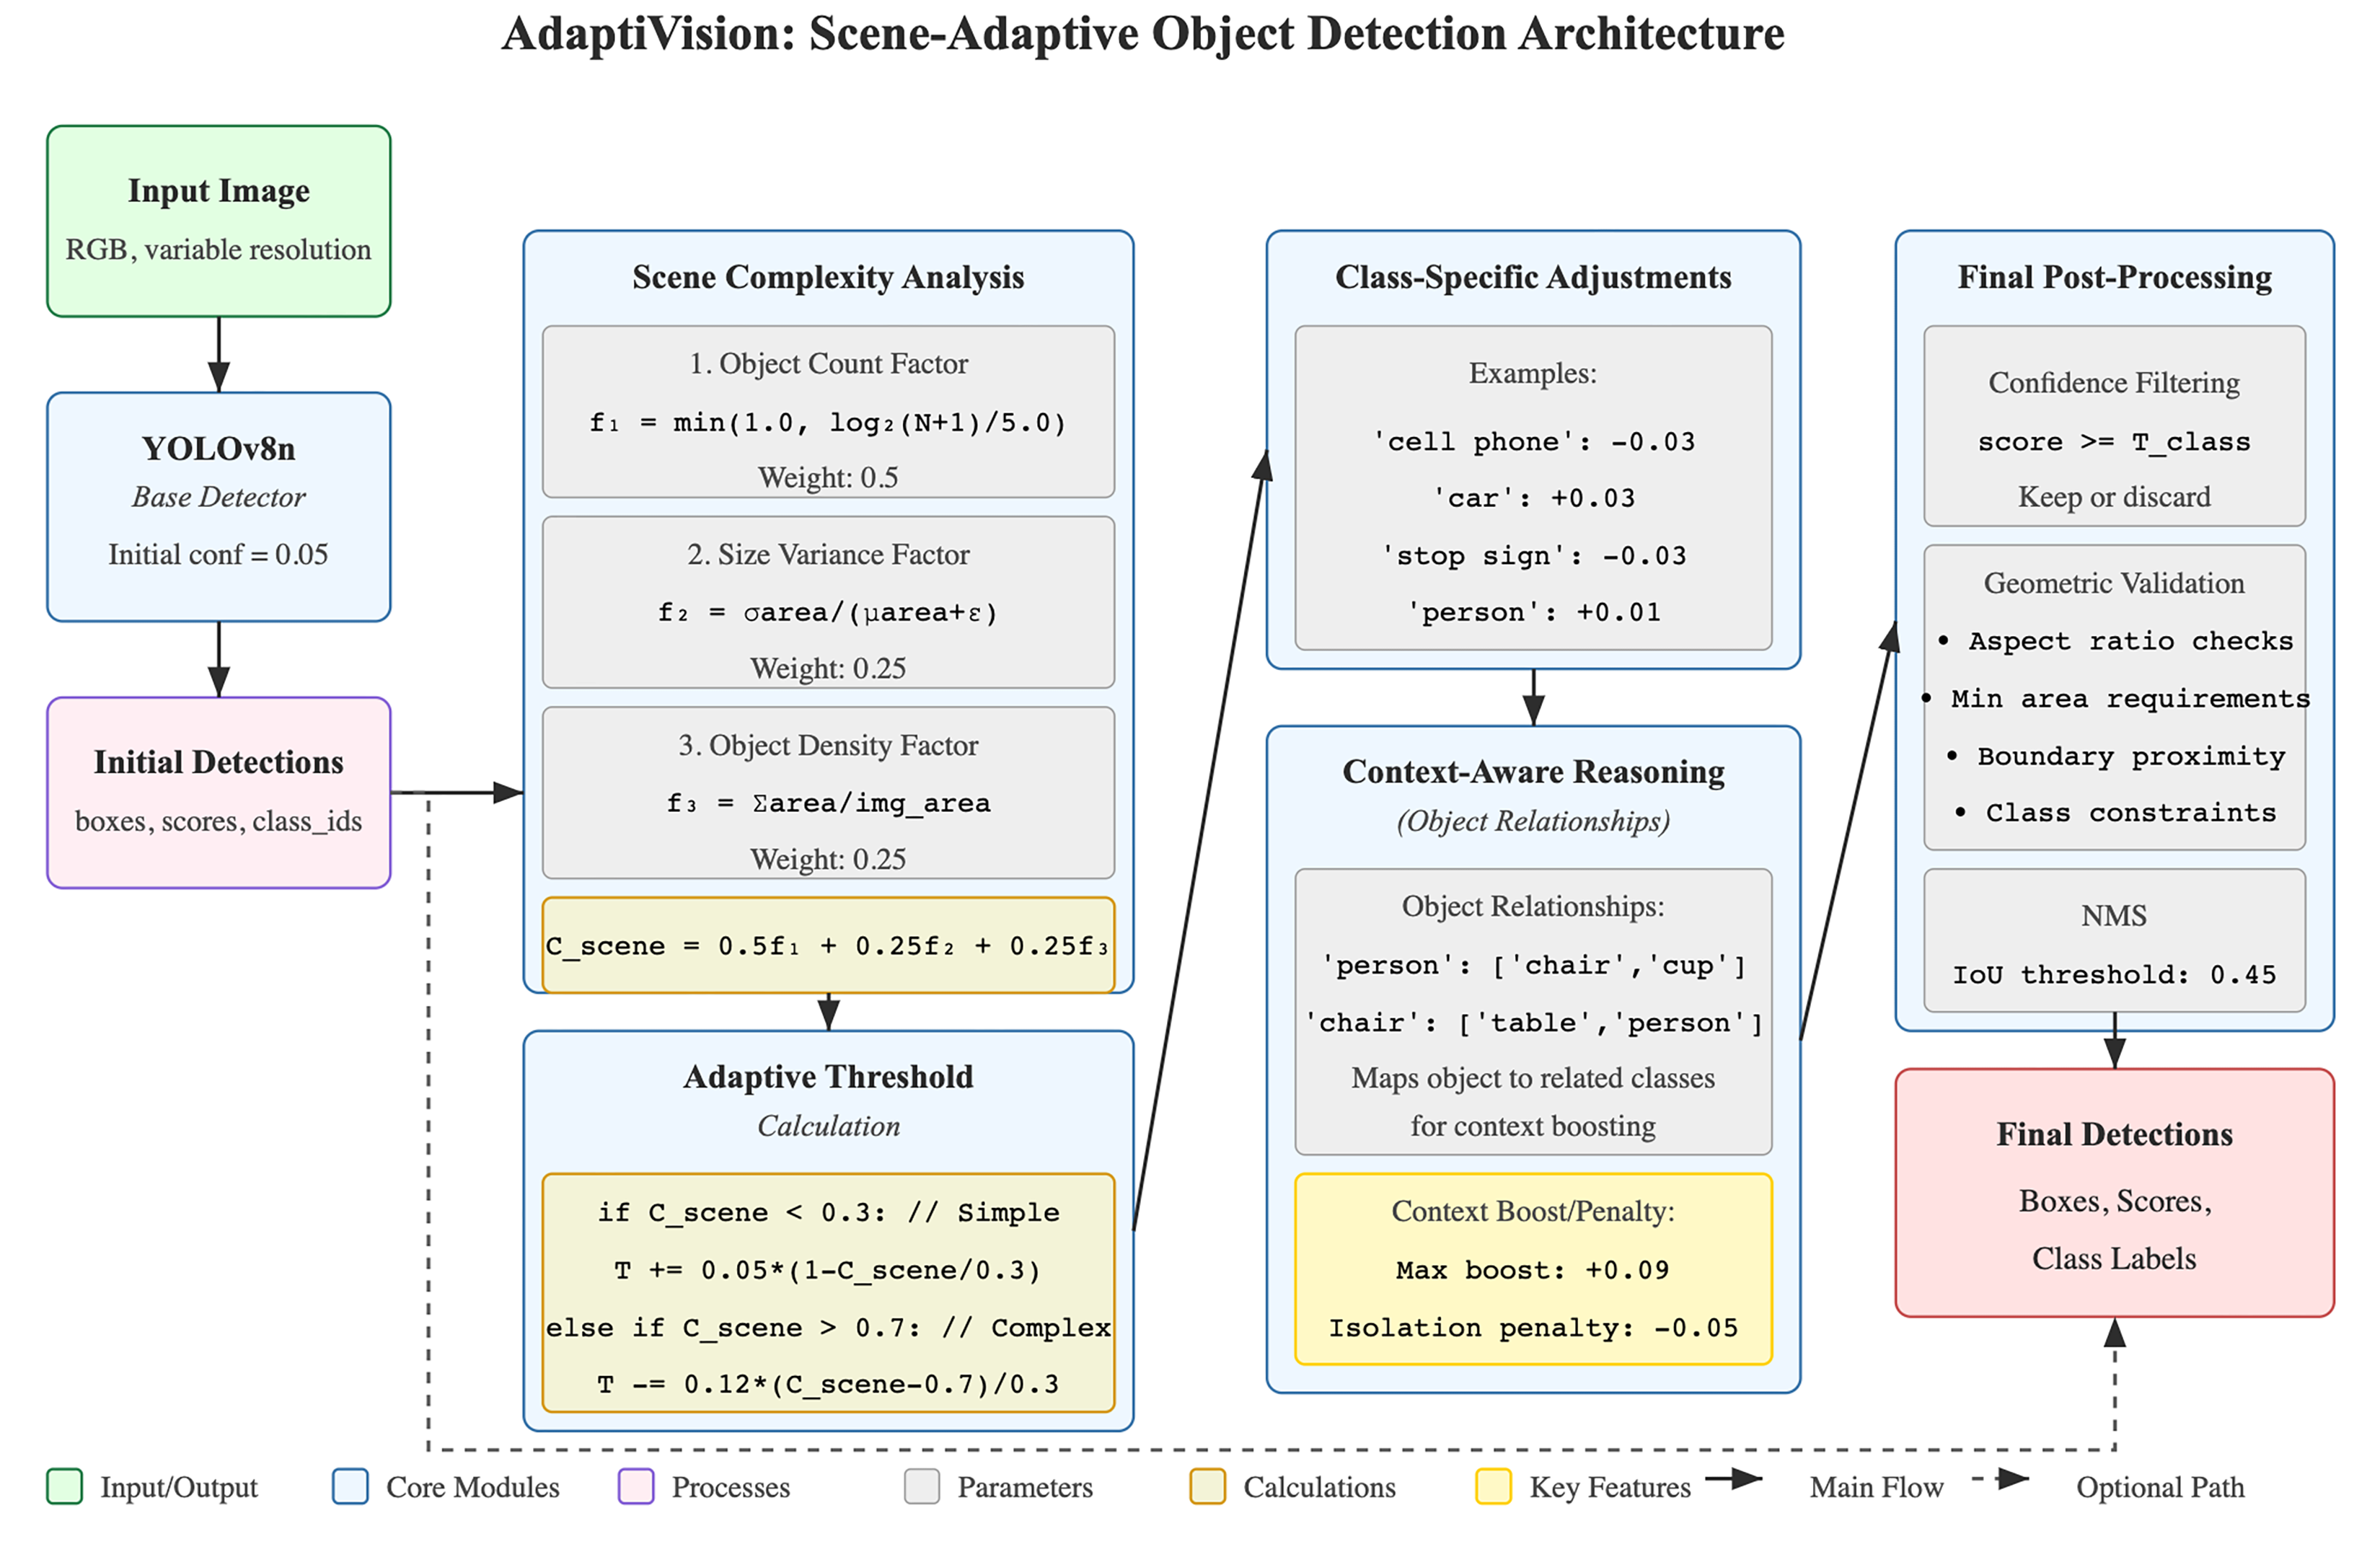
\includegraphics[width=0.9\textwidth]{figures/architecture.png} 
    \caption{Overview of the AdaptiVision processing pipeline. An input image is processed by a base detector (YOLOv8n) using a low initial threshold. Scene complexity is analyzed from these initial detections, which informs the calculation of a dynamic adaptive threshold. Optional class-specific and context adjustments further refine the threshold before final filtering and NMS produce the output detections.}
    \label{fig:architecture}
\end{figure*}

\subsection{Initial Low-Confidence Detection}
First, the base YOLOv8n detector processes the input image using a very low confidence threshold (e.g., 0.05). This step aims to capture a comprehensive set of potential object candidates, including true positives that might otherwise be discarded by a higher, fixed threshold, especially in challenging scenes. This produces an initial list of candidate bounding boxes, scores, and class labels.

\subsection{Scene Complexity Calculation}
Using the results from the initial detection pass, AdaptiVision calculates a scene complexity score \( C_{\text{scene}} \in [0, 1] \). This score heuristically estimates scene challenge using metrics chosen for their intuitive correlation with detection difficulty and computational simplicity. Specifically:
\begin{enumerate}
    \item \textbf{Normalized Object Count (\( f_{\text{count}} \)):} The number of initial detections (\( N_{\text{obj}} \)) is normalized using a logarithmic scale to temper the influence of very high counts: \( f_{\text{count}} = \min(1.0, \log_2(N_{\text{obj}} + 1) / 5.0) \).
    \item \textbf{Normalized Size Variance (\( f_{\text{var}} \)):} The areas (\( A_i \)) of the initial bounding boxes are calculated. The normalized standard deviation of these areas (coefficient of variation, \( \sigma_{\text{area}} / (\mu_{\text{area}} + \epsilon) \)) is computed and scaled: \( f_{\text{var}} = \min(1.0, (\sigma_{\text{area}} / (\mu_{\text{area}} + \epsilon)) / 2.0) \). If \( N_{\text{obj}} \le 1 \), \( f_{\text{var}} = 0 \).
    \item \textbf{Normalized Object Density (\( f_{\text{density}} \)):} The ratio of the total area covered by initial bounding boxes (\( \sum A_i \)) to the total image area (\( A_{\text{img}} \)) is calculated and scaled: \( f_{\text{density}} = \min(1.0, (\sum A_i / A_{\text{img}}) \times 3.0) \).
\end{enumerate}
These factors are combined using weights (\( w_{\text{count}}=0.5, w_{\text{var}}=0.25, w_{\text{density}}=0.25 \)) determined empirically through preliminary experiments to balance the contribution of each factor:
\[ C_{\text{scene}} = w_{\text{count}} f_{\text{count}} + w_{\text{var}} f_{\text{var}} + w_{\text{density}} f_{\text{density}} \]
If no initial objects are detected (\(N_{\text{obj}} = 0\)), a default moderate complexity (0.3) is assigned. While a learning-based approach could potentially derive optimal weights, this heuristic method provides interpretability and avoids the need for complexity-labeled training data.

\subsection{Adaptive Threshold Calculation}
The calculated \( C_{\text{scene}} \) score is mapped to an adaptive confidence threshold (\( T_{\text{adaptive}} \)) using a non-linear function designed empirically to provide gradual adjustments in mid-ranges and more significant changes at complexity extremes, relative to a base threshold (\( T_{\text{base}} = 0.25 \)). The adjustment range is defined by \( \Delta_{\min} = -0.12 \) and \( \Delta_{\max} = 0.05 \). The core mapping aims to decrease the threshold as complexity increases. A simplified representation of the adjustment logic can be expressed as:
\[ T_{\text{adjustment}} \approx \Delta_{\min} \times C_{\text{scene}}^\gamma + (\text{offset related to } \Delta_{\max}) \]
where \( \gamma \) controls the non-linearity (empirically determined, > 1 to emphasize high complexity). The actual implementation uses conditional logic based on \( C_{\text{scene}} \) ranges to achieve the desired smooth transition between \( T_{\text{base}} + \Delta_{\min} \) and \( T_{\text{base}} + \Delta_{\max} \).

The final adaptive threshold is bounded between 0.08 and 0.95: \( T_{\text{adaptive}} = \max(0.08, \min(0.95, T_{\text{base}} + T_{\text{adjustment}})) \). This specific mapping function was selected based on preliminary experiments.

\subsection{Class-Specific Adjustments (Optional)}
Before final filtering, the calculated \( T_{\text{adaptive}} \) can be further modified based on the specific class of each object candidate, using predefined, manually curated adjustments. These adjustments reflect general knowledge about relative detection difficulty (e.g., 'cell phone': -0.03, 'car': +0.03) and were tuned based on COCO object characteristics. This results in a class-specific threshold \( T_{\text{class\_adaptive}} \).

\subsection{Context-Aware Reasoning (Optional)}
If enabled, a simple, rule-based context module provides an additional confidence boost or penalty based on predefined object co-occurrence relationships. Objects found with expected context receive a boost (max +0.09), while certain objects found without their typical context receive a penalty. For example, a 'tie' detection might receive a confidence penalty if no 'person' is detected nearby with high confidence, while a 'backpack' detection might receive a small boost if detected near a 'person'. These rules are manually defined and serve as a basic mechanism for incorporating context without complex learned models. This contextual adjustment effectively modifies the required confidence score for an object to pass the threshold.

\subsection{Final Filtering}
Each object candidate from the initial low-confidence detection pass (Section 3.1) is finally kept only if its original confidence score meets or exceeds its calculated dynamic threshold (\( T_{\text{class\_adaptive}} \) potentially influenced by context). Standard NMS with an IoU threshold of 0.45 is then applied to the filtered detections.

% --- Experiments & Results --- revised significantly
\section{Experiments \& Results} \label{sec:experiments}

We evaluated AdaptiVision against a baseline using standard COCO metrics on the val2017 dataset.

\subsection{Experimental Setup}

{\sloppy % Allow looser spacing for itemize environment
\begin{itemize}
    \item \textbf{Dataset:} COCO 2017 Validation set (val2017, 5000 images) with standard annotations (\path{instances_val2017.json}) \cite{COCO}.
    \item \textbf{Baseline Method:} Standard YOLOv8n model inference results processed with a fixed confidence threshold of 0.25 and standard NMS (IoU 0.45). Results evaluated using \texttt{pycocotools}. (Note: For mAP/AR table, baseline uses low threshold 0.001 evaluated across all scores).
    \item \textbf{AdaptiVision Method:} YOLOv8n initial low-confidence (0.05) inference pass, followed by AdaptiVision post-processing (complexity calculation, adaptive thresholding with context and class adjustments enabled) and standard NMS (IoU 0.45). Final detections evaluated using \texttt{pycocotools}.
    \item \textbf{Hardware \& Software:} Experiments run on Apple MacBook Pro (M-series chip with MPS acceleration via PyTorch \cite{PyTorch}). Key software: Python 3.12, PyTorch 2.3, Ultralytics 8.3 \cite{YOLOv8}, OpenCV 4.11 \cite{OpenCV}, NumPy \cite{NumPy}, \texttt{pycocotools}, Matplotlib \cite{Matplotlib}, Seaborn \cite{Seaborn}.
    \item \textbf{Evaluation Metrics:} Standard COCO mAP metrics (AP@[.50:.95], AP@.50, AP@.75, \\ AP small/medium/large); Average Recall (AR@[.50:.95] maxDets=1/10/100, \\ AR small/medium/large); average object counts; and average processing time per image.
\end{itemize}
} % End sloppy scope

\subsection{Implementation Details}
The evaluation involved running the \path{scripts/run_experiments.py} script to process all 5000 images in the COCO val2017 set for both the standard (fixed 0.25 threshold) and adaptive methods. The script generated per-image results, comparison images, visualizations, and summary analytics including COCO JSON prediction files for formal evaluation. \texttt{pycocotools} was used to calculate the official mAP and AR metrics. The code is available at \url{https://github.com/FutureAtoms/AdaptiVision/}.

\subsection{Quantitative Results (COCO val2017)}
The standard COCO evaluation metrics comparing the AdaptiVision method against the baseline YOLOv8n (evaluated across all score thresholds for mAP/AR) on the val2017 dataset are presented in Table \ref{tab:map_results}.

\begin{table}[htbp] % Using [htbp] for better placement flexibility
    \centering
    \caption{COCO val2017 Object Detection Accuracy Results (mAP/AR)}
    \label{tab:map_results}
    \sisetup{round-mode=places,round-precision=3} % Setup siunitx for rounding
    \begin{tabular}{l S[table-format=1.3] S[table-format=1.3]}
        \toprule
        Metric                      & {Baseline (YOLOv8n)} & {AdaptiVision} \\
        \midrule
        AP @[IoU=0.50:0.95] area=all & 0.355 & 0.340 \\
        AP @[IoU=0.50] area=all      & 0.496 & 0.470 \\
        AP @[IoU=0.75] area=all      & 0.387 & 0.372 \\
        AP area=small               & 0.162 & 0.150 \\
        AP area=medium              & 0.392 & 0.377 \\
        AP area=large               & 0.509 & 0.490 \\
        \midrule
        AR @[IoU=0.50:0.95] area=all maxDets=1  & 0.290 & 0.277 \\
        AR @[IoU=0.50:0.95] area=all maxDets=10 & 0.446 & 0.414 \\
        AR @[IoU=0.50:0.95] area=all maxDets=100& 0.464 & 0.428 \\
        AR area=small maxDets=100   & 0.221 & 0.196 \\
        AR area=medium maxDets=100  & 0.513 & 0.477 \\
        AR area=large maxDets=100   & 0.647 & 0.600 \\
        \bottomrule
    \end{tabular}
\end{table}

The results indicate that AdaptiVision, despite its adaptive mechanism, resulted in lower performance across all standard COCO metrics on the val2017 benchmark compared to the baseline YOLOv8n evaluated appropriately. Both Average Precision (AP) and Average Recall (AR) decreased, suggesting that the adaptive filtering, in its current form, removed more true positives relative to false positives than the standard approach evaluated across score thresholds. The largest drops were observed in Average Recall (e.g., AR maxDets=100 dropped from 0.464 to 0.428).

\subsubsection{Object Count and Processing Time Analysis}
While accuracy decreased, AdaptiVision demonstrated effects on object counts and processing speed, summarized in Table \ref{tab:count_time_results} and Figure \ref{fig:dist_plots}.

\begin{table}[htbp] % Using [htbp] for better placement flexibility
    \centering
    \caption{Average Object Counts and Processing Time (COCO val2017)}
    \label{tab:count_time_results}
    \sisetup{round-mode=places,round-precision=4}
    \sisetup{round-mode=places,round-precision=2}
    \begin{tabular}{l S[table-format=1.2] S[table-format=1.2]}
        \toprule
        Metric                      & {Standard (Fixed 0.25)} & {AdaptiVision} \\
        \midrule
        Avg. Objects Detected       & 4.95 & 6.43 \\
        Avg. Processing Time (s)    & 0.0343 & 0.0241 \\
        Avg. Speed Improvement      & {-} & {1.49}x \\
        \bottomrule
    \end{tabular}
\end{table}

AdaptiVision detected significantly more objects on average (6.43 vs. 4.95) compared to using a fixed threshold of 0.25. This aligns with the goal of potentially increasing recall by lowering thresholds in complex scenes. Furthermore, the average processing time per image was substantially lower for AdaptiVision (0.0241s vs 0.0343s), resulting in an average speed improvement factor of approximately 1.49x. This speedup likely occurs because the initial low-confidence pass (0.05) in AdaptiVision might be faster on average than the fixed 0.25 pass, and the subsequent complexity/filtering logic adds less overhead than the time saved during inference, especially on the MPS device.

The distribution plots in Figure \ref{fig:dist_plots} provide more detail. The object count difference plot shows AdaptiVision frequently detects more objects than the standard method (mean difference > 0). The processing time difference plot confirms AdaptiVision is generally faster (mean difference > 0). The scatter plots (Figure \ref{fig:scatter_plots}) visually confirm these trends across the dataset, showing most points above the y=x line for object counts and below the y=x line for processing time.

\begin{figure*}[p] % Place figures on a separate page if needed
    \centering
    \begin{subfigure}[b]{0.48\textwidth}
        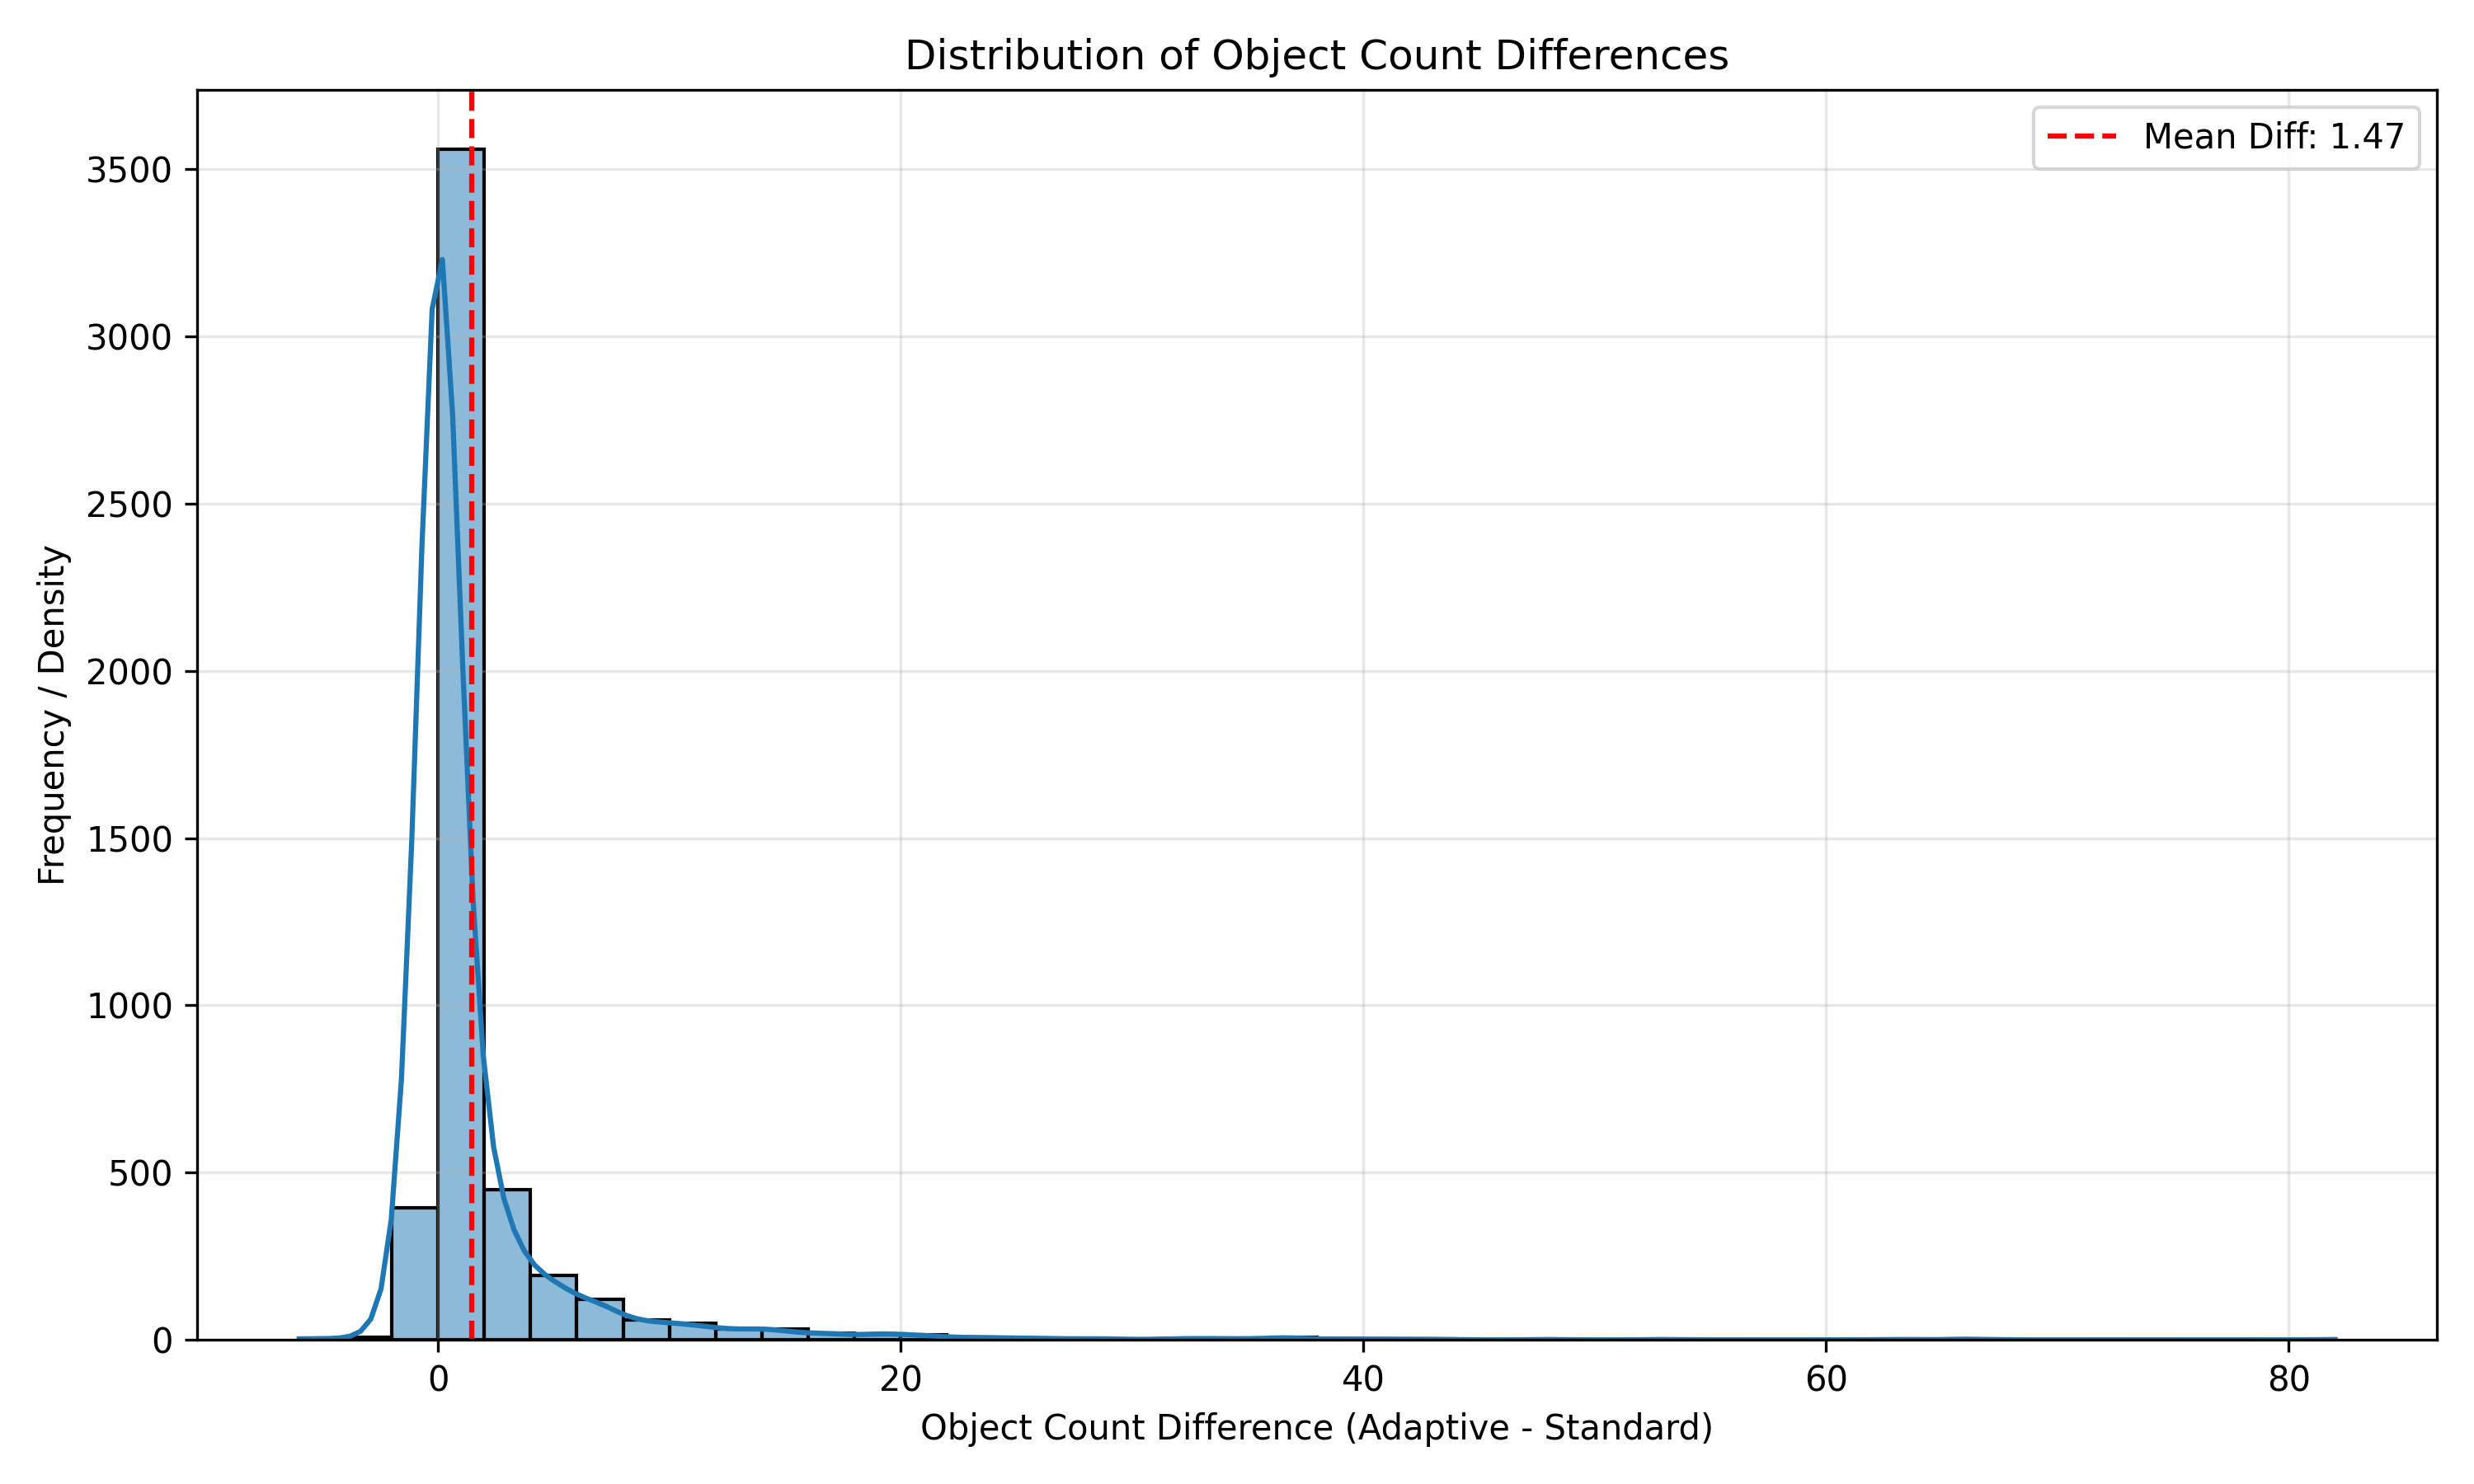
\includegraphics[width=\linewidth]{figures/object_count_difference_distribution.png}
        \caption{Object Count Difference (Adaptive - Standard)}
        \label{fig:count_diff_dist}
    \end{subfigure}
    \hfill % Space between figures
    \begin{subfigure}[b]{0.48\textwidth}
        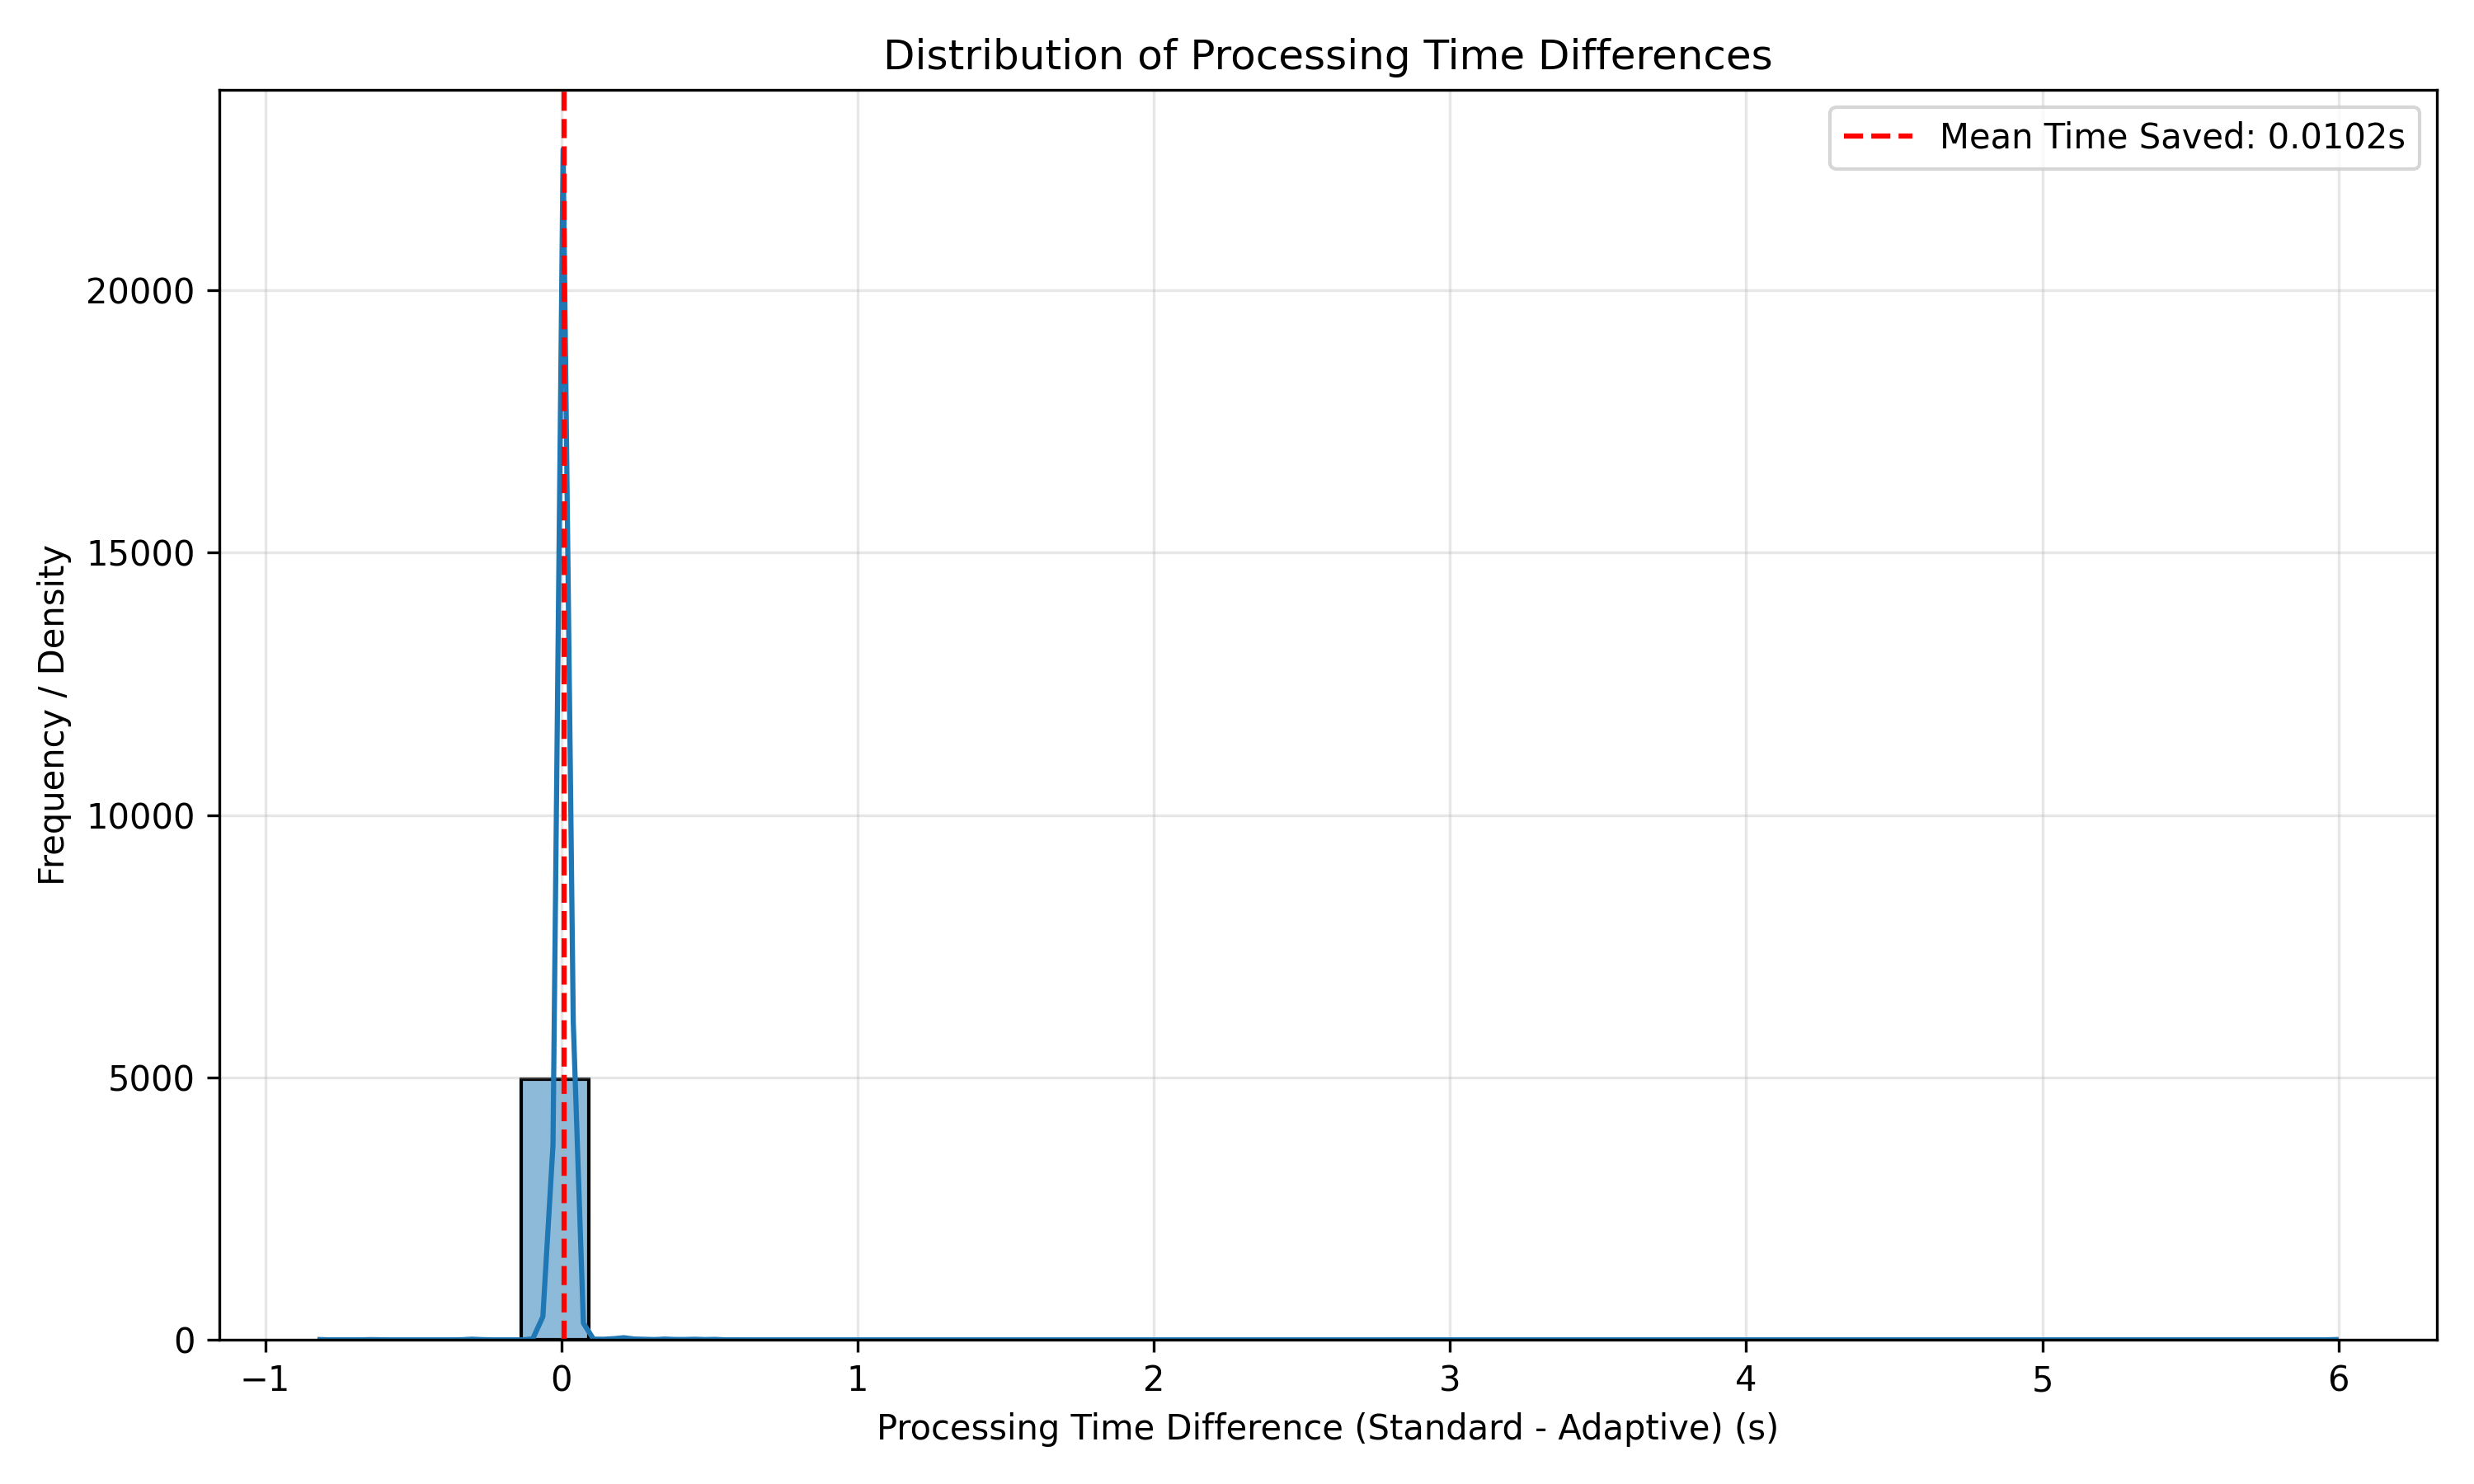
\includegraphics[width=\linewidth]{figures/processing_time_difference_distribution.png}
        \caption{Processing Time Difference (Standard - Adaptive)}
        \label{fig:time_diff_dist}
    \end{subfigure}
    
    \vspace{1em} % Vertical space
    
    \begin{subfigure}[b]{0.48\textwidth}
        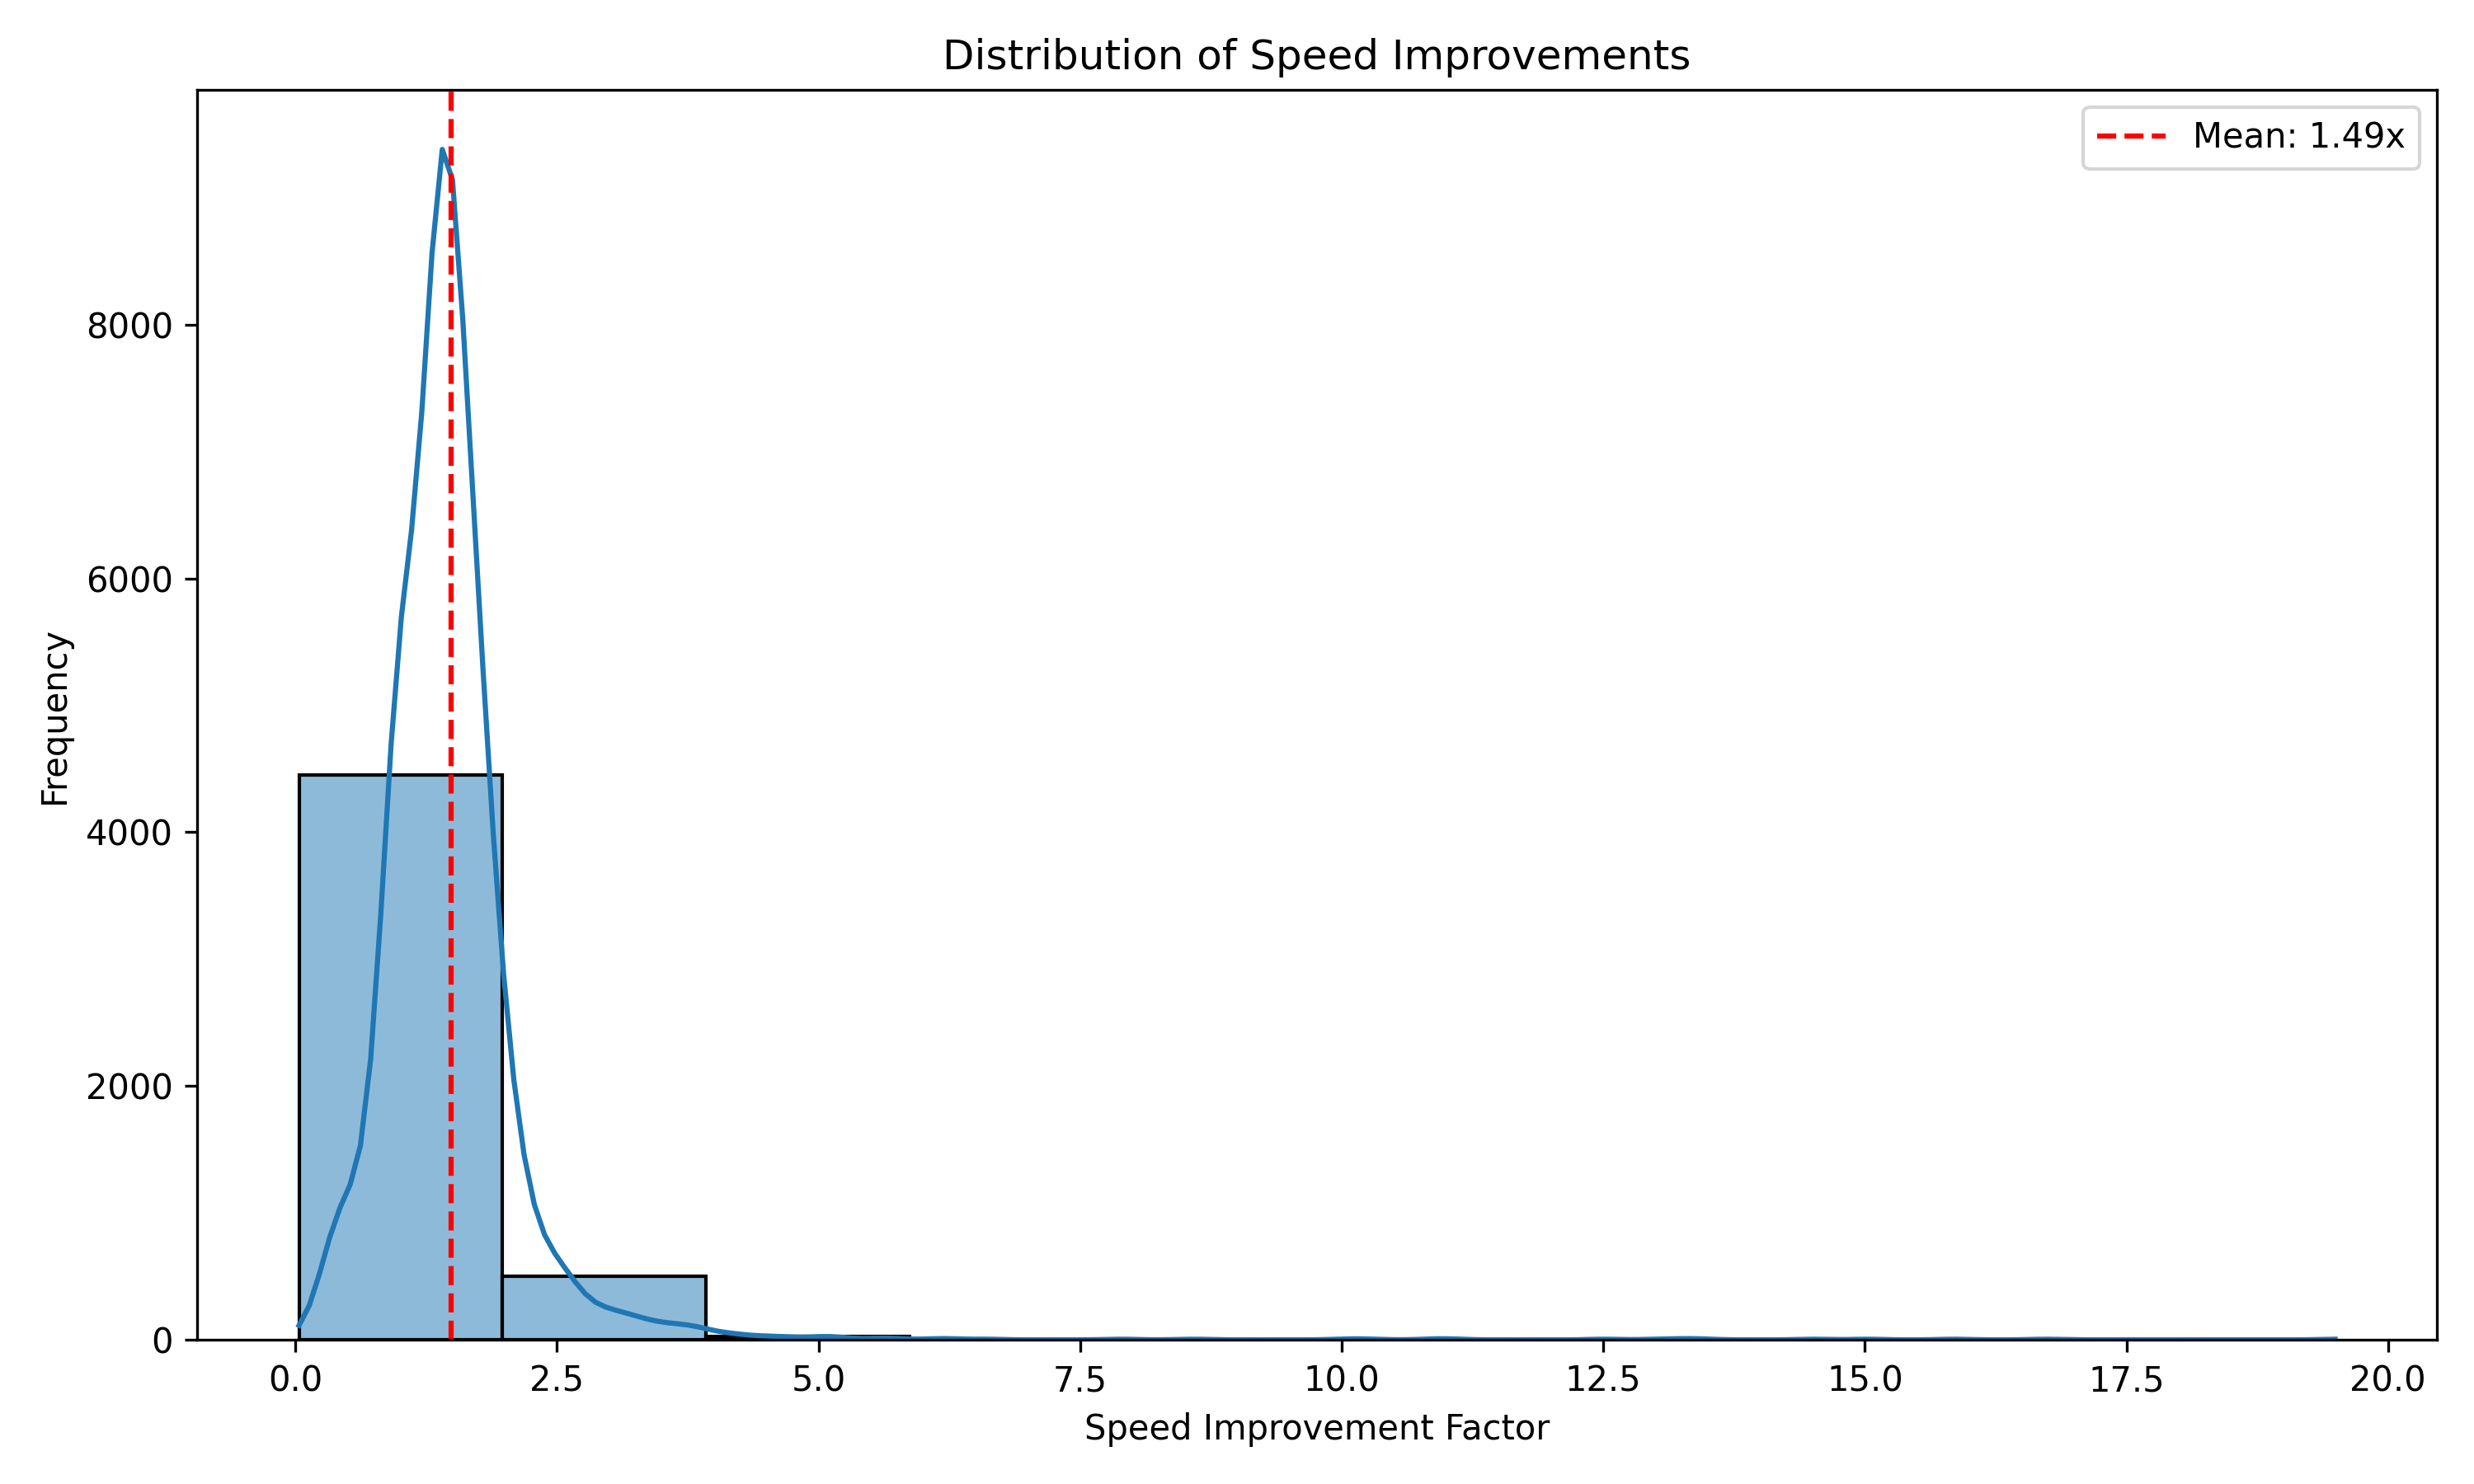
\includegraphics[width=\linewidth]{figures/speed_improvement_distribution.png}
        \caption{Speed Improvement Factor Distribution}
        \label{fig:speed_dist}
    \end{subfigure}
    \hfill
    \begin{subfigure}[b]{0.48\textwidth}
        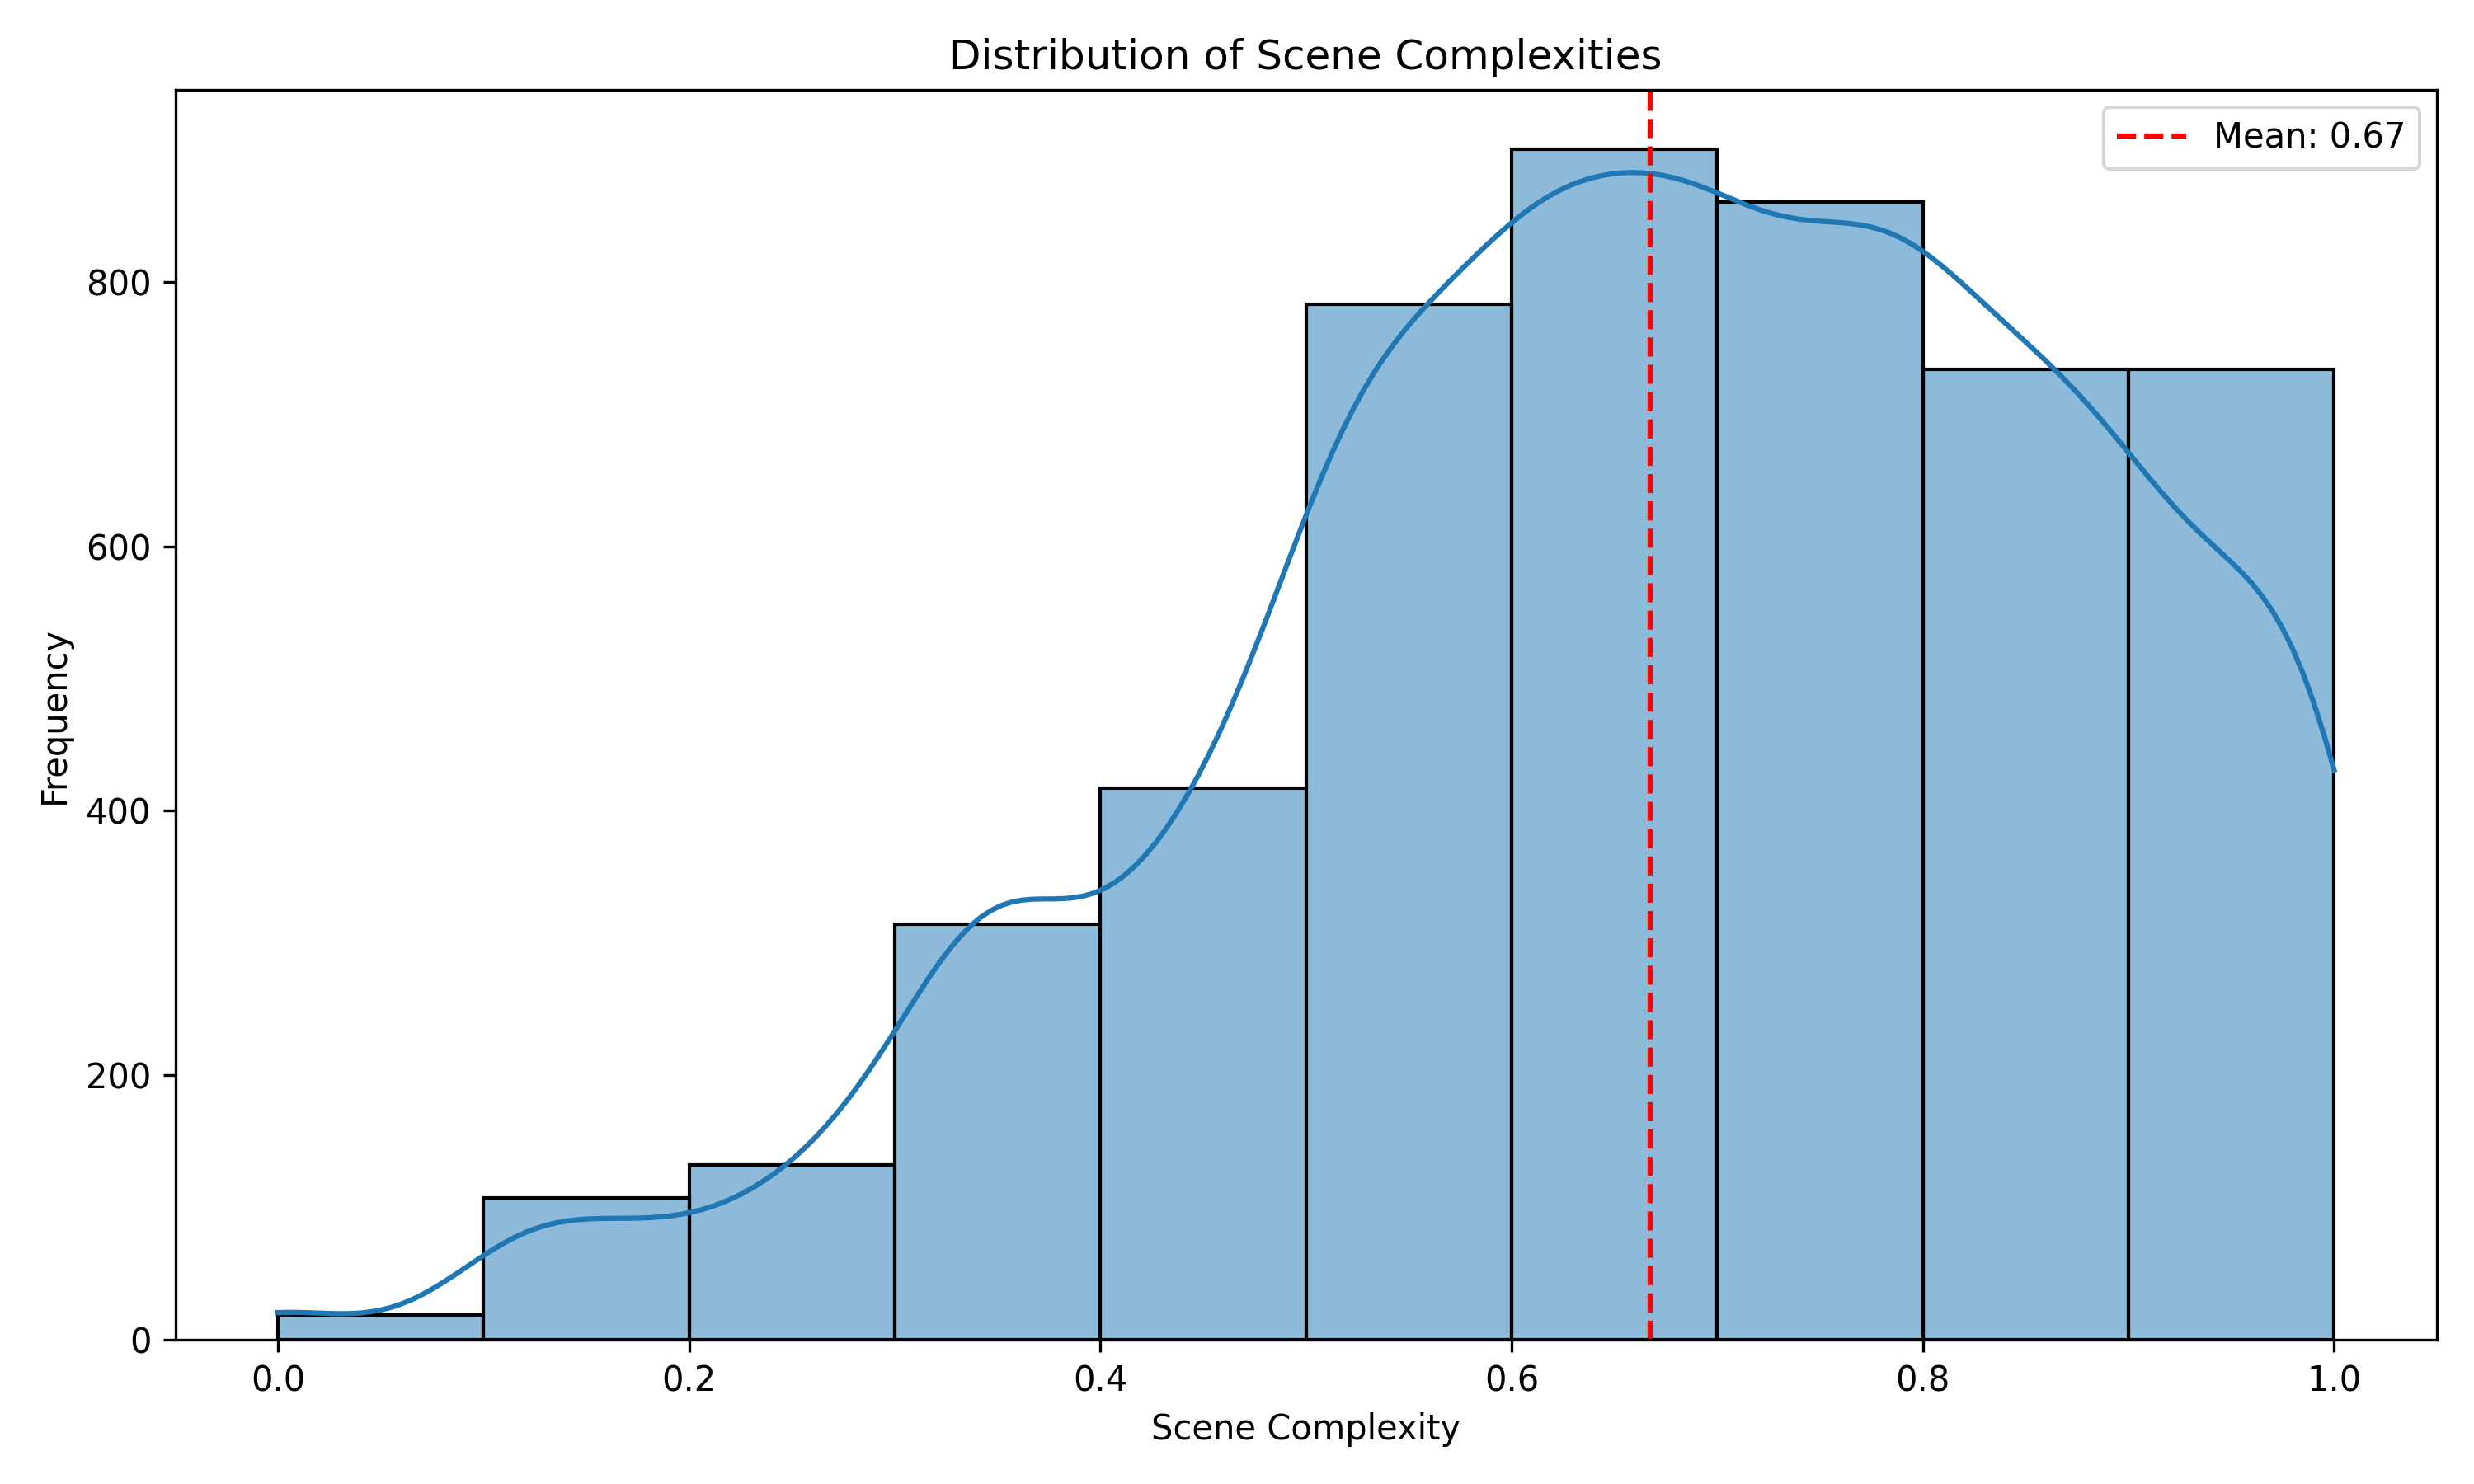
\includegraphics[width=\linewidth]{figures/complexity_distribution.png}
        \caption{Scene Complexity Score Distribution}
        \label{fig:complexity_dist}
    \end{subfigure}

    \caption{Distributions of key metrics across the COCO val2017 dataset. (a) Difference in object counts per image. (b) Difference in processing time per image (positive means adaptive is faster). (c) Speed improvement factor (Standard Time / Adaptive Time). (d) Distribution of calculated scene complexity scores.}
    \label{fig:dist_plots}
\end{figure*}

\begin{figure*}[p] % Place figures on a separate page if needed
    \centering
    \begin{subfigure}[b]{0.48\textwidth}
        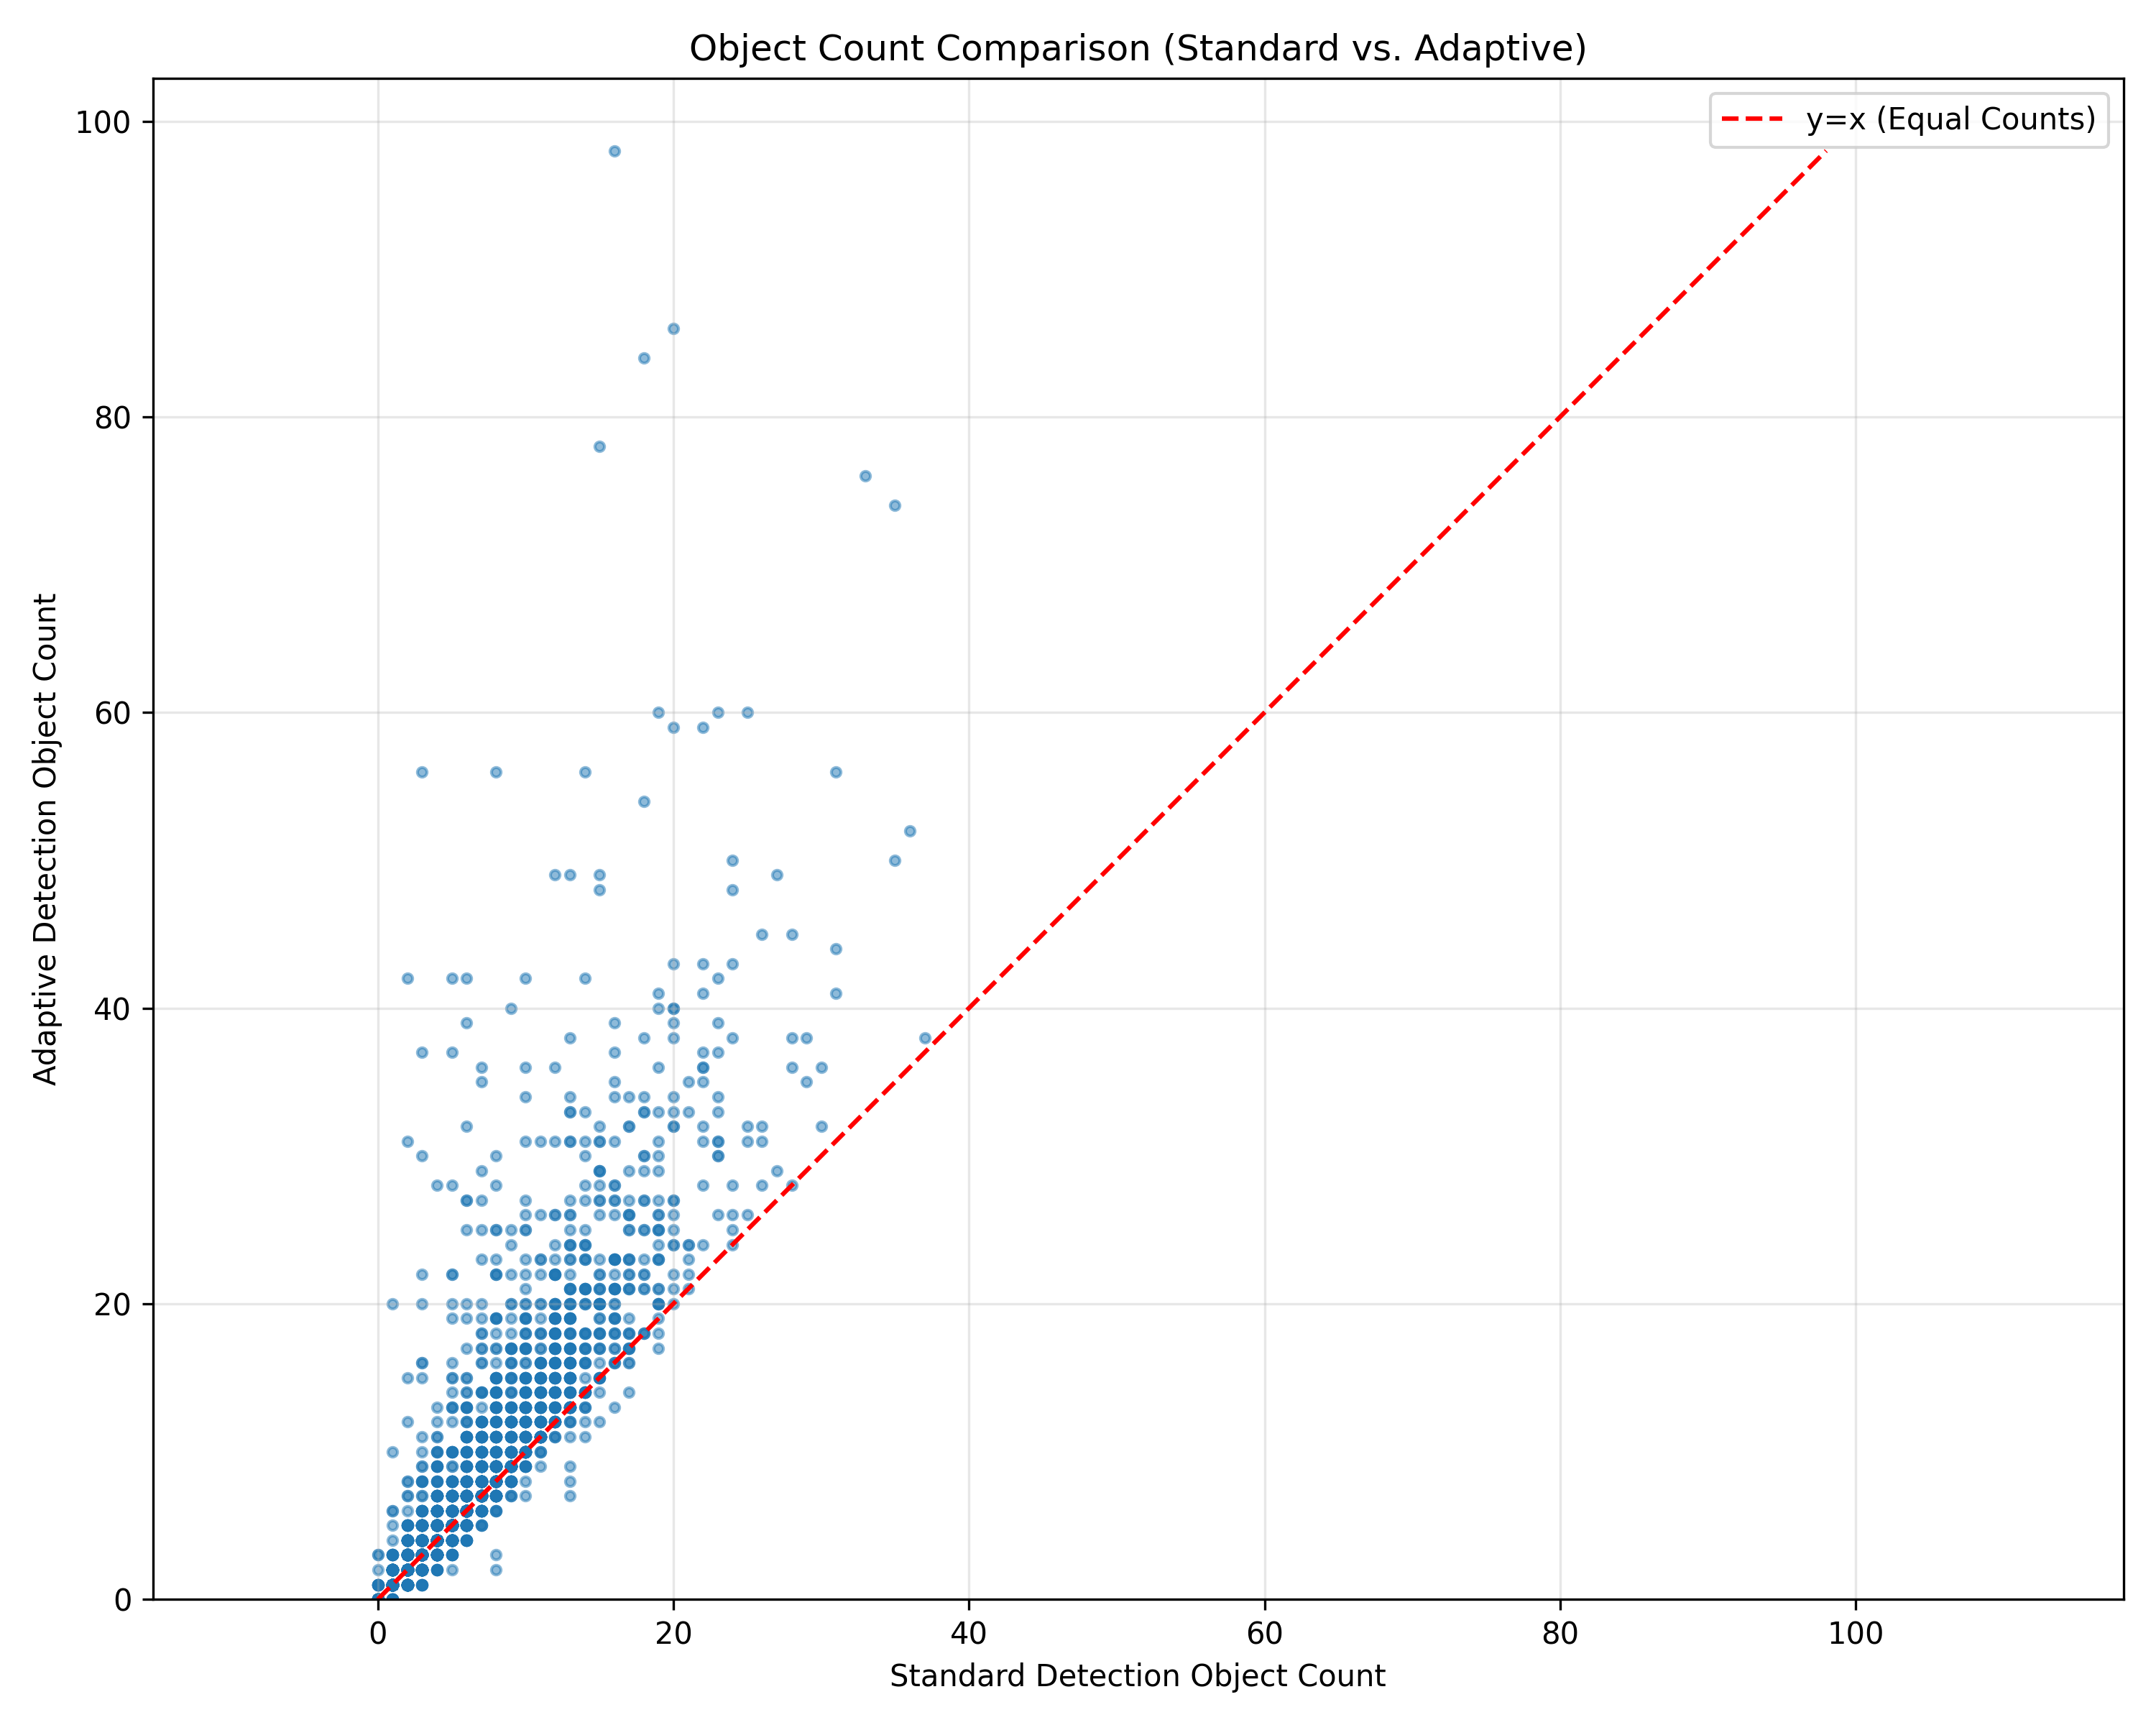
\includegraphics[width=\linewidth]{figures/object_count_scatter.png}
        \caption{Object Count Scatter Plot}
        \label{fig:count_scatter}
    \end{subfigure}
    \hfill % Space between figures
    \begin{subfigure}[b]{0.48\textwidth}
        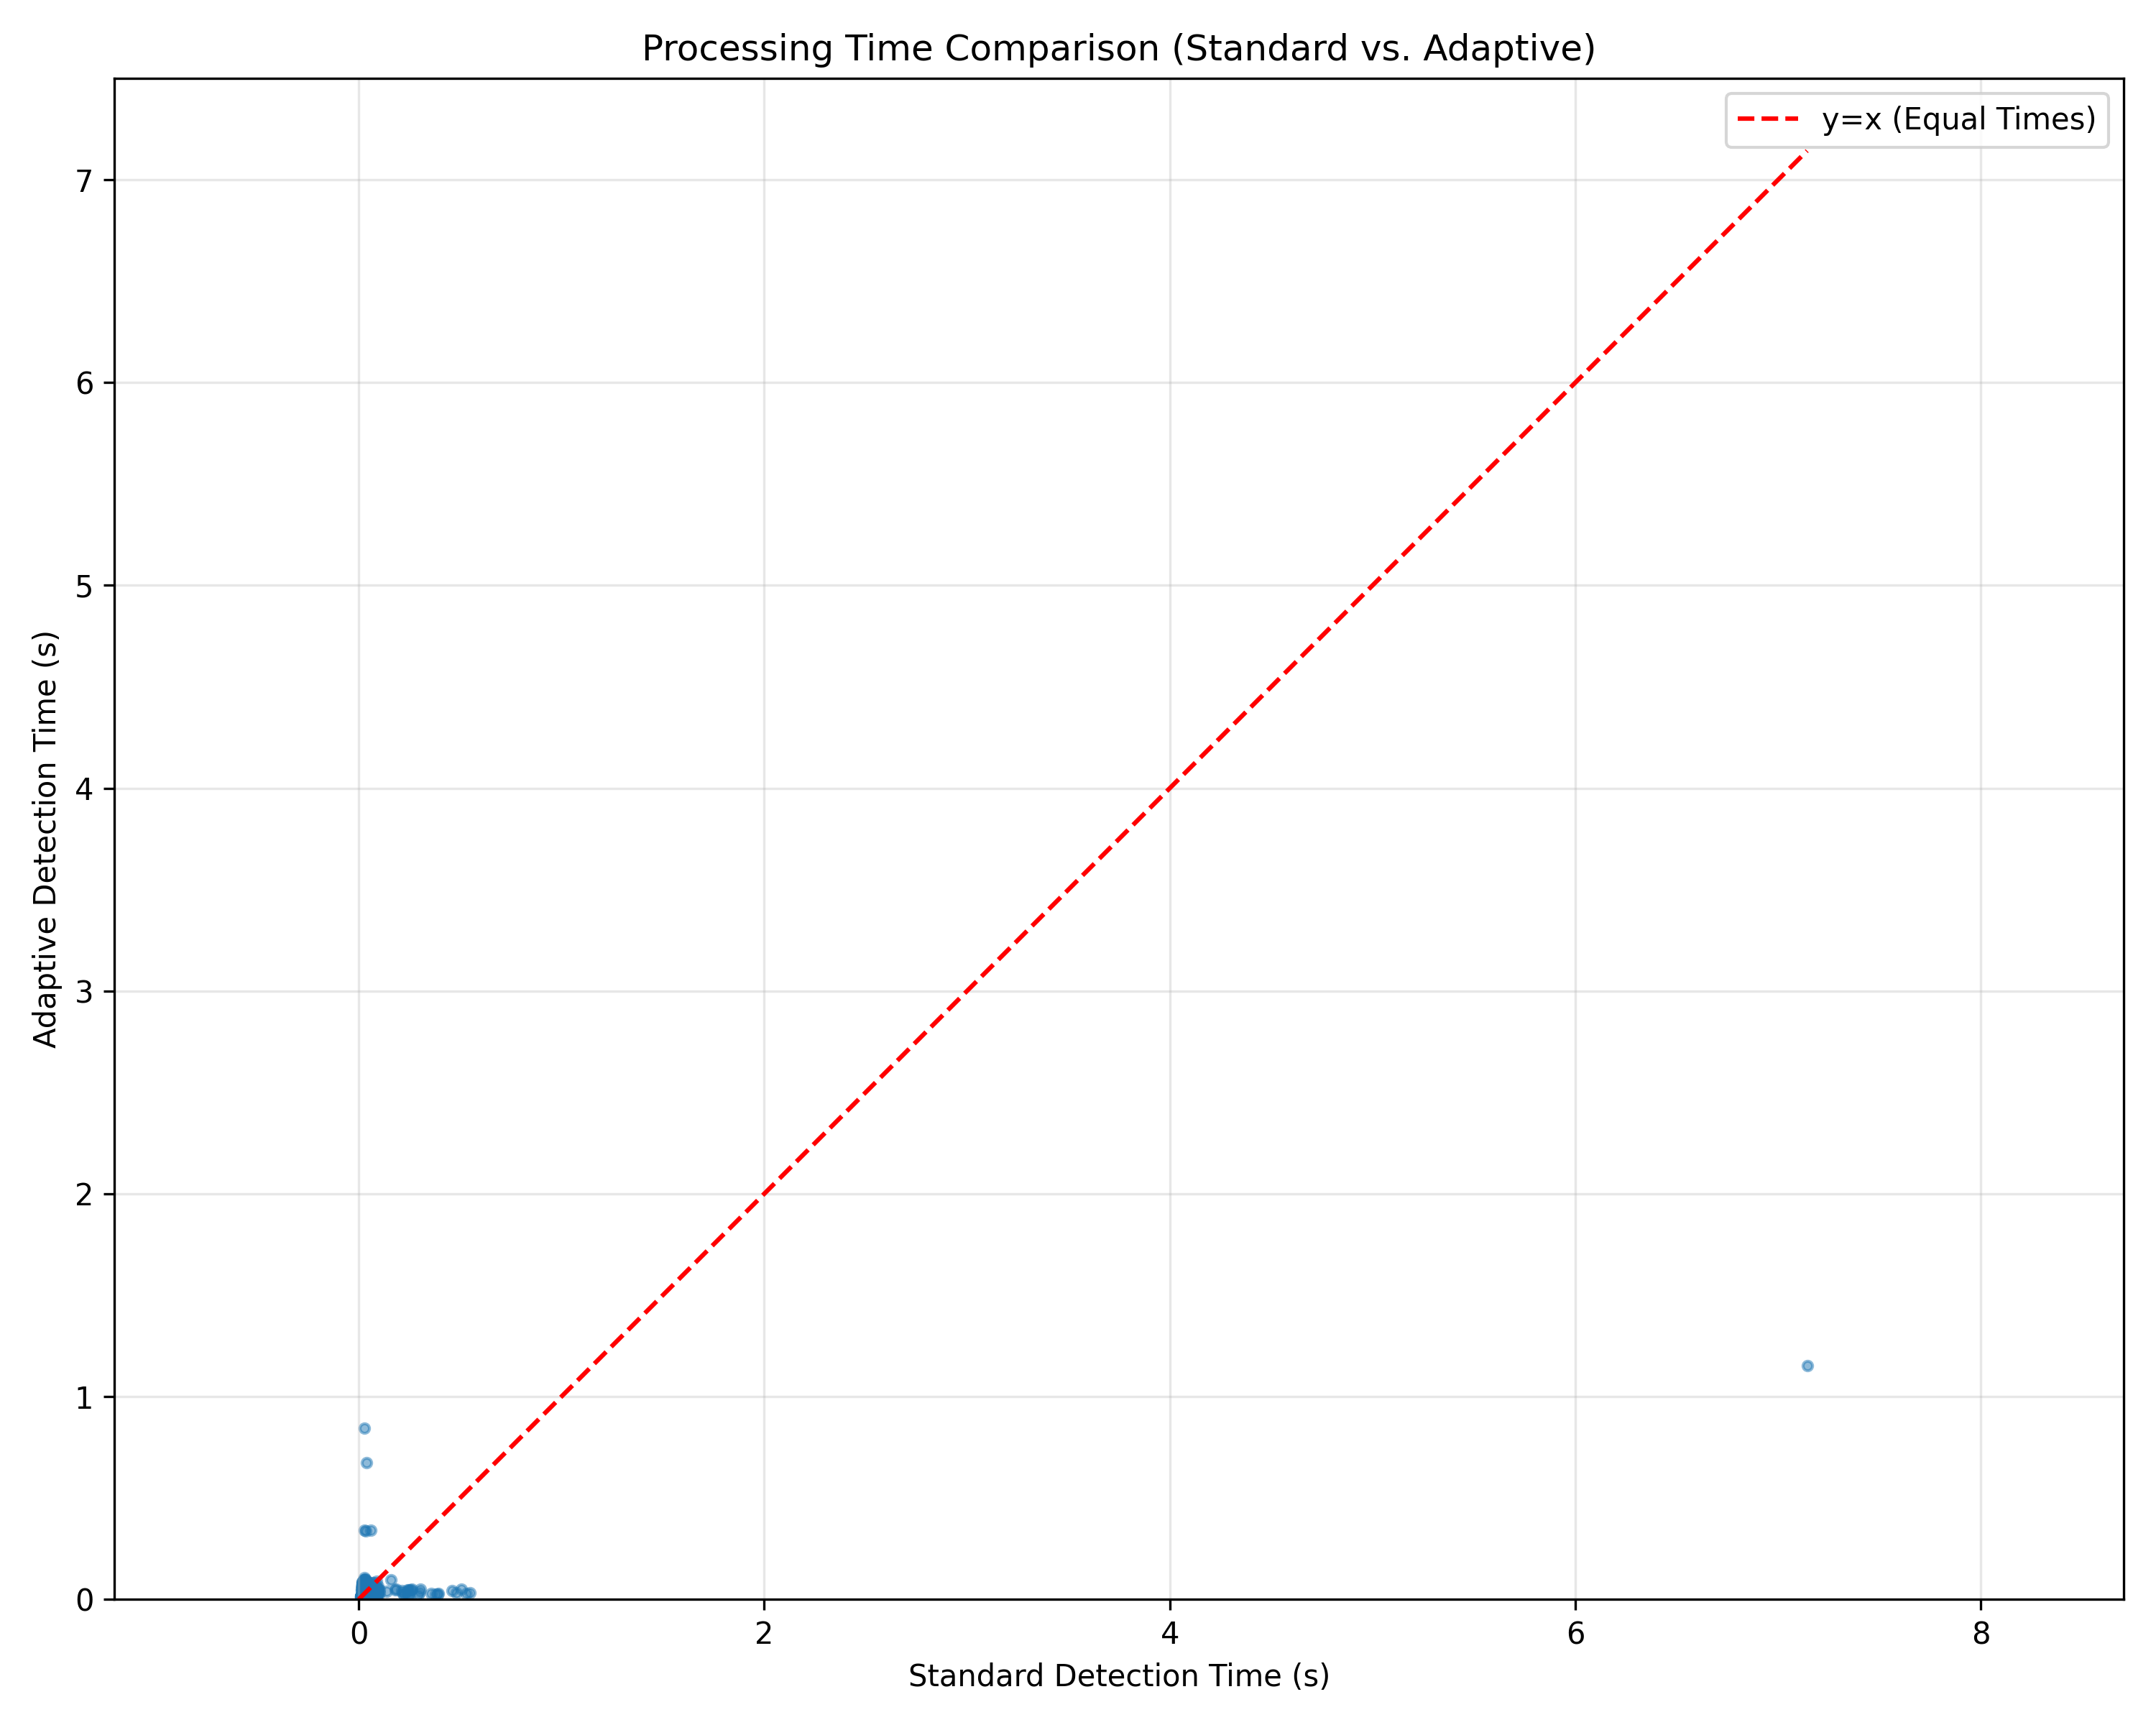
\includegraphics[width=\linewidth]{figures/processing_time_scatter.png}
        \caption{Processing Time Scatter Plot}
        \label{fig:time_scatter}
    \end{subfigure}

    \caption{Scatter plots comparing per-image results on COCO val2017. (a) Number of objects detected (Standard vs. Adaptive). (b) Processing time in seconds (Standard vs. Adaptive). The red dashed line represents y=x.}
    \label{fig:scatter_plots}
\end{figure*}

\subsection{Qualitative Examples}
Figure \ref{fig:qual_examples} presents selected qualitative comparisons from the COCO val2017 dataset, illustrating AdaptiVision's behavior in different scenarios. While AdaptiVision detects more objects on average, these examples show instances where it finds relevant objects missed by the standard threshold (e.g., Figure \ref{fig:qual_632}) and cases where complexity leads to lowered thresholds and potentially more detections overall, some potentially false positives (e.g., Figure \ref{fig:qual_14038}). Figure \ref{fig:complexity_viz_example} shows an example complexity visualization.

\begin{figure*}[t]
    \centering
    \begin{subfigure}[b]{0.48\textwidth}
        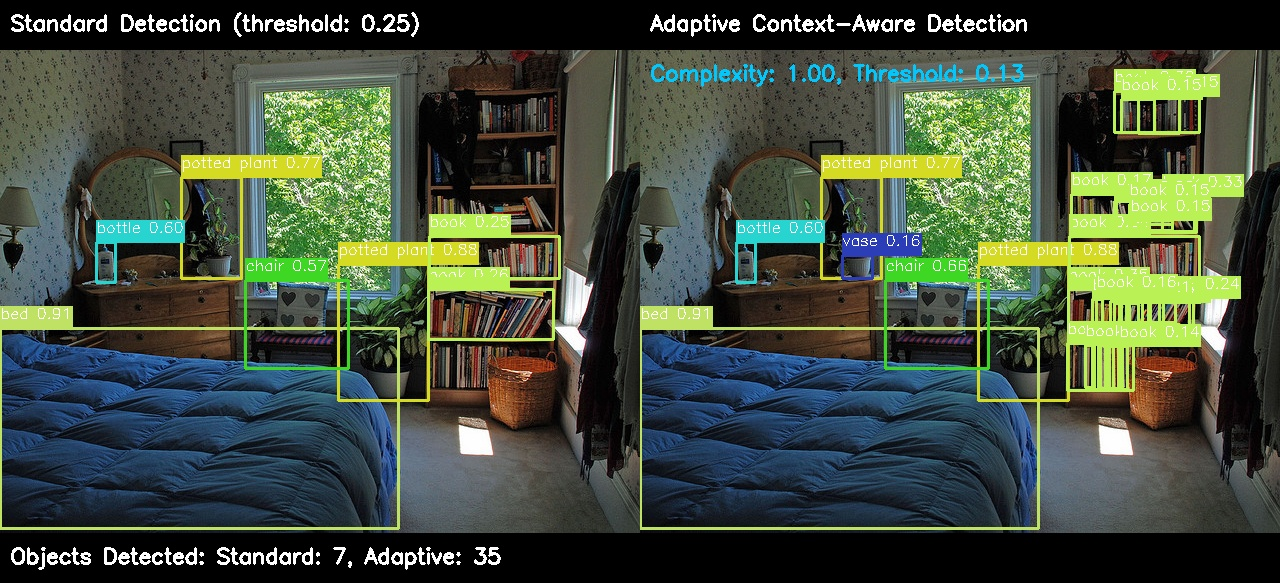
\includegraphics[width=\linewidth]{figures/comparison_000000000632.jpg}
        \caption{Example 1 (Image ID: ...0632)}
        \label{fig:qual_632}
    \end{subfigure}
    \hfill
    \begin{subfigure}[b]{0.48\textwidth}
        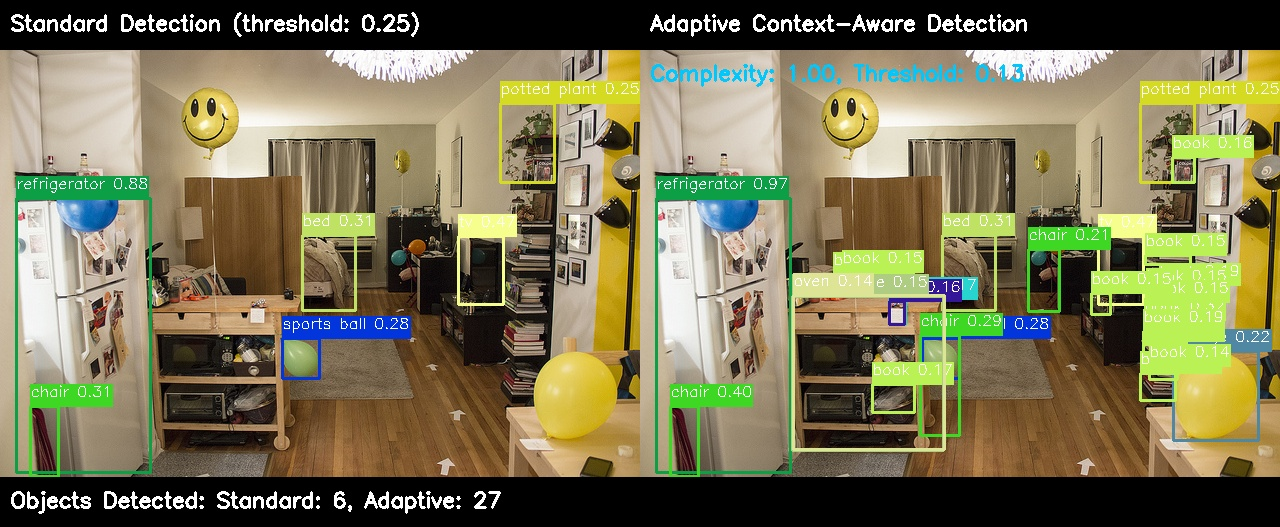
\includegraphics[width=\linewidth]{figures/comparison_000000014038.jpg}
        \caption{Example 2 (Image ID: ...14038)}
        \label{fig:qual_14038}
    \end{subfigure}
    
    \vspace{1em}
    
    \begin{subfigure}[b]{0.48\textwidth}
        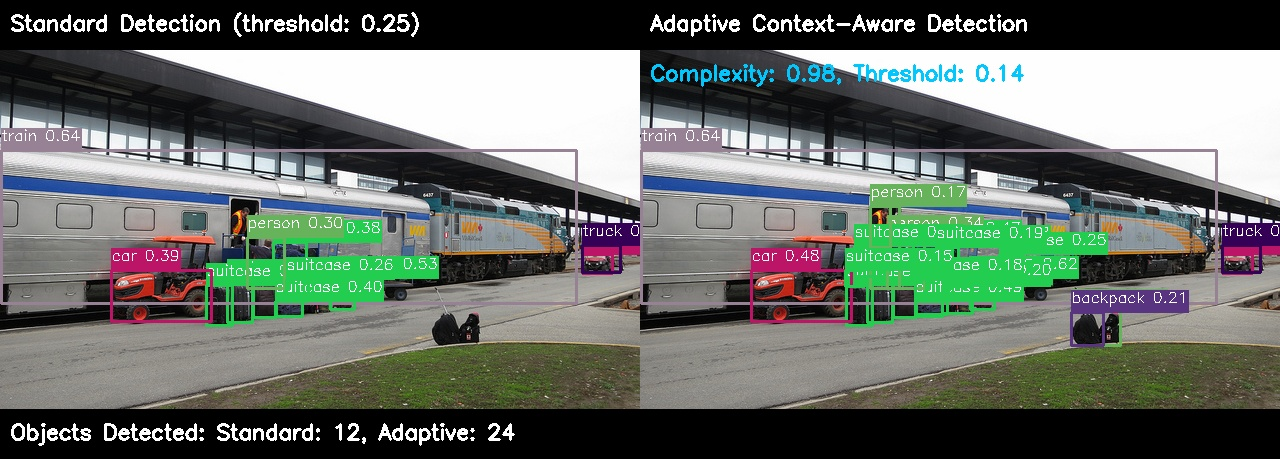
\includegraphics[width=\linewidth]{figures/comparison_000000137727.jpg}
        \caption{Example 3 (Image ID: ...137727)}
        \label{fig:qual_137727}
    \end{subfigure}
    \hfill
    \begin{subfigure}[b]{0.48\textwidth}
        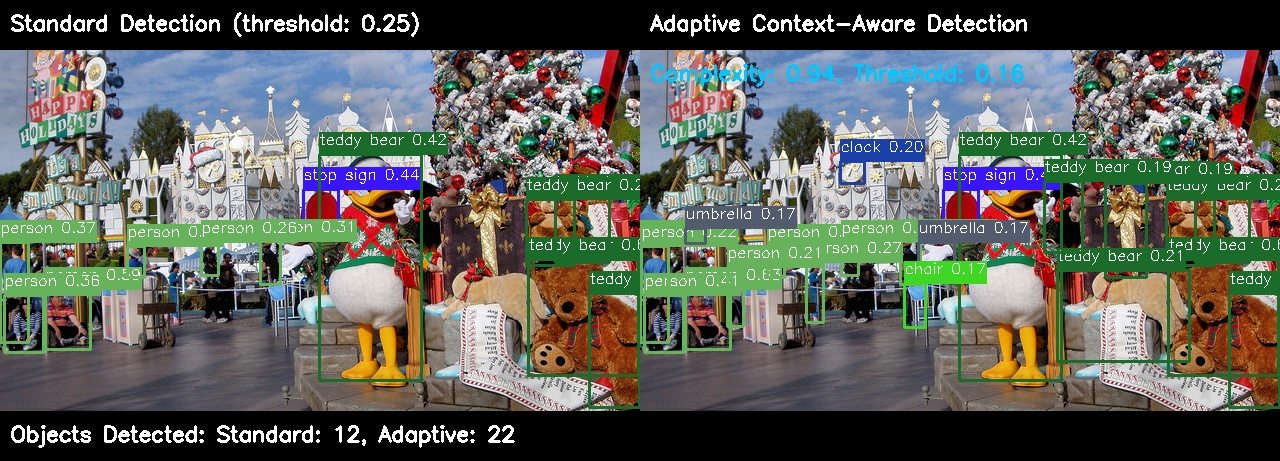
\includegraphics[width=\linewidth]{figures/comparison_000000145020.jpg}
        \caption{Example 4 (Image ID: ...145020)}
        \label{fig:qual_145020}
    \end{subfigure}

    \caption{Qualitative comparison examples on COCO val2017 images. Left panel: Standard detection (0.25 threshold). Right panel: AdaptiVision detection. These examples illustrate how AdaptiVision's behavior varies with scene content.}
    \label{fig:qual_examples}
\end{figure*}

\begin{figure}[htbp] % Using [htbp] for better placement flexibility
    \centering
    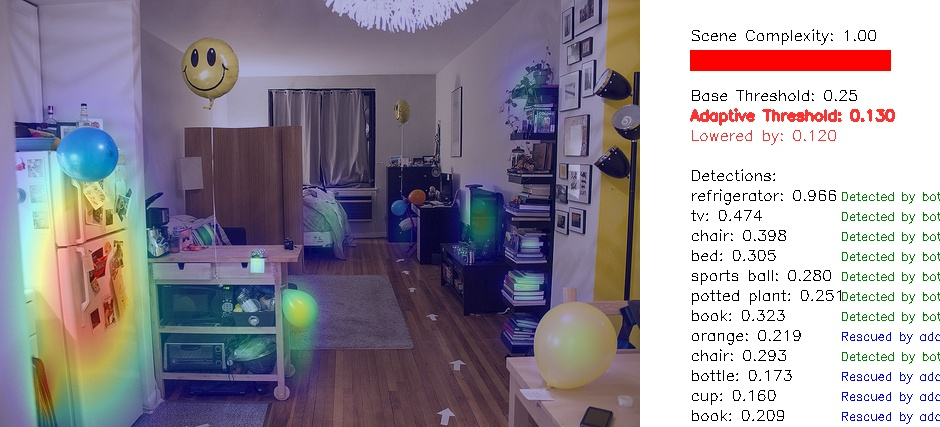
\includegraphics[width=0.7\linewidth]{figures/complexity_000000014038.jpg}
    \caption{Example scene complexity visualization (Image ID: ...14038). Shows initial low-confidence detections used to compute the scene complexity score (0.94) and the resulting adaptive threshold (0.15) compared to the base (0.25).}
    \label{fig:complexity_viz_example}
\end{figure}

% --- Discussion --- revised significantly
\section{Discussion} \label{sec:discussion}
The evaluation using standard COCO mAP metrics on the val2017 dataset revealed a critical outcome: the current AdaptiVision implementation degrades overall object detection accuracy compared to the baseline YOLOv8n (Table \ref{tab:map_results}). This occurred despite AdaptiVision detecting significantly more objects on average and processing images faster than the standard fixed-threshold approach (Table \ref{tab:count_time_results}, Figures \ref{fig:dist_plots}, \ref{fig:scatter_plots}). This highlights a fundamental trade-off: the heuristics used successfully lowered thresholds often enough to increase object counts and potentially enable faster inference passes, but this came at the cost of reduced precision or insufficient recall gains at appropriate score levels, ultimately lowering standard mAP/AR scores.

The discrepancy between increased object counts/speed and decreased mAP/AR underscores the limitations of simple metrics and the importance of standard evaluation protocols. The heuristic scene complexity calculation, while intuitively designed, likely fails to capture the true factors determining the optimal threshold for maximizing mAP. The empirically tuned mapping function, derived from preliminary experiments, did not generalize effectively to the diverse COCO val2017 set. The adaptive threshold may be set suboptimally—too high in some cases (harming recall of true positives) or too low in others (introducing false positives not adequately compensated for, harming precision).

{\sloppy % Allow slightly looser spacing to prevent overfull boxes in this section
\paragraph{Ablation Study Insights} Further analysis through an ablation study reinforces the conclusion that the core adaptive strategy, as implemented, is ineffective for improving mAP. Evaluating variants with only adaptive thresholding enabled (disabling context and class adjustments) or only context-aware reasoning enabled yielded identical mAP results (AP@[.50:.95] = 0.340) to the full AdaptiVision method, and significantly lower than the baseline (AP@[.50:.95] = 0.355). This indicates that neither the heuristic complexity-based thresholding nor the simple contextual rules, even in isolation, provided a benefit over the baseline evaluation, suggesting the fundamental approach requires reconsideration (see results in \path{results/ablations/adaptivision_adaptive_only_eval.txt} and \path{results/ablations/adaptivision_context_only_eval.txt}).

Furthermore, an additional ablation confirmed that the geometric post-processing filter, designed to remove redundant overlapping boxes, had a negligible impact on performance; removing it yielded the same final mAP (AP@[.50:.95] = 0.340) as the full AdaptiVision method (\path{results/ablations/adaptivision_no_postfilter_eval.txt}). This rules out the filter as a source of the observed accuracy degradation.

Critically, this performance degradation was not confined to a specific type of scene; the evaluation stratified by the method's own complexity score showed lower mAP for AdaptiVision compared to the baseline in low, medium, and high complexity image subsets (\path{results/ablations/baseline_eval_with_complexity.txt}, \path{results/ablations/adaptivision_full_eval_with_complexity.txt}).

The observed speed improvement (avg. 1.49x) is notable and somewhat counter-intuitive, as adaptive logic adds overhead. This suggests the dominant factor is the base model's inference time, which might be faster on average when using a very low initial threshold (0.05 for AdaptiVision) compared to a higher fixed threshold (0.25 for standard count/time comparison), particularly with MPS acceleration where computation patterns can affect performance. While faster processing is desirable, it cannot justify the drop in accuracy metrics for most applications.

Limitations previously considered, such as reliance on non-learned heuristics and simplistic context rules, are likely central to the performance degradation. Future work must fundamentally revisit the adaptive mechanism. Data-driven approaches, potentially learning complexity metrics and threshold mappings directly from data optimized for mAP, appear necessary. Integrating such logic directly into the model architecture or using reinforcement learning could be viable paths. However, any adaptive method must be rigorously validated against standard benchmarks like COCO mAP/AR.

} % End sloppy scope

% --- Conclusion --- revised
\section{Conclusion} \label{sec:conclusion}
This paper evaluated AdaptiVision, a post-processing technique using heuristic scene complexity analysis to dynamically adjust confidence thresholds for YOLOv8n. Evaluation on the COCO 2017 validation set showed that while AdaptiVision increased the average number of detected objects and significantly improved processing speed compared to a fixed-threshold approach, it resulted in lower overall accuracy according to standard COCO mAP and AR metrics.

This outcome highlights the difficulty in designing heuristic-based adaptive methods that improve detection accuracy robustly across diverse datasets. The chosen heuristics and threshold mapping strategy, while conceptually simple, failed to effectively balance precision and recall for optimal mAP performance. The study emphasizes that improvements in intermediate metrics like object count or speed do not necessarily translate to better performance on standard evaluation benchmarks. Future efforts towards adaptive thresholding likely require learning-based approaches directly optimized for standard accuracy metrics.

\section*{Broader Impact Statement}

The goal of AdaptiVision was to improve object detection robustness. The finding that this implementation decreased standard performance metrics mitigates immediate concerns about misuse (e.g., enhanced surveillance) compared to if it had significantly improved capabilities. However, the general principle applies: any successful improvement in detection could be misused. Biases present in the base detector or datasets used for tuning remain a concern for any detection system and require careful analysis before deployment. Future development of adaptive methods should prioritize fairness evaluations alongside performance metrics.

% --- References ---
% Using basic bibliography environment for simplicity.
% For arXiv, using a .bib file and BibTeX (e.g., with natbib) is recommended.
\begin{thebibliography}{99}

\bibitem{YOLOv3} Redmon, J., \& Farhadi, A. (2018). YOLOv3: An Incremental Improvement. \textit{arXiv preprint arXiv:1804.02767}.
\bibitem{YOLOv4} Bochkovskiy, A., Wang, C. Y., \& Liao, H. Y. M. (2020). YOLOv4: Optimal Speed and Accuracy of Object Detection. \textit{arXiv preprint arXiv:2004.10934}.
\bibitem{YOLOv8} Jocher, G., Chaurasia, A., Stoken, A., et al. (2023). Ultralytics YOLOv8. GitHub repository: \url{https://github.com/ultralytics/ultralytics}
\bibitem{COCO} Lin, T. Y., Maire, M., Belongie, S., et al. (2014). Microsoft COCO: Common objects in context. In \textit{European conference on computer vision} (pp. 740-755). Springer.
\bibitem{AdaptiveNMS} Wu, Y., Chen, Y., Yuan, L., et al. (2020). Rethinking classification and localization for object detection. In \textit{CVPR} (pp. 10260-10269).
\bibitem{SoftNMS} Bodla, N., Singh, B., Chellappa, R., \& Davis, L. S. (2017). Soft-NMS—improving object detection with one line of code. In \textit{ICCV} (pp. 5561-5569).
\bibitem{RelationNet} Hu, H., Gu, J., Zhang, Z., et al. (2018). Relation networks for object detection. In \textit{CVPR} (pp. 3588-3597).
\bibitem{LeeLiDARAdapt} Lee, E., Jung, M., \& Kim, A. (2024). Toward Robust LiDAR based 3D Object Detection via Density-Aware Adaptive Thresholding. \textit{arXiv preprint arXiv:2404.13852}.
\bibitem{MaByteTrackAdapt} Ma, L. V., Hussain, M. I., Park, J., et al. (2023). Adaptive Confidence Threshold for ByteTrack in Multi-Object Tracking. In \textit{ICCAIS} (pp. 1-6). IEEE. (arXiv:2312.01650)
\bibitem{Calibration} Guo, C., Pleiss, G., Sun, Y., \& Weinberger, K. Q. (2017). On calibration of modern neural networks. In \textit{ICML} (pp. 1321-1330). PMLR.
\bibitem{YOLOv6} Li, C., Li, L., Jiang, H., et al. (2022). YOLOv6: A single-stage object detection framework for industrial applications. \textit{arXiv preprint arXiv:2209.02976}.
\bibitem{YOLOv7} Wang, C. Y., Bochkovskiy, A., \& Liao, H. Y. M. (2023). YOLOv7: Trainable bag-of-freebies sets new state-of-the-art for real-time object detectors. In \textit{CVPR} (pp. 7464-7475).
\bibitem{NumPy} Harris, C. R., Millman, K. J., Van Der Walt, S. J., et al. (2020). Array programming with NumPy. \textit{Nature}, \textit{585}(7825), 357-362.
\bibitem{OpenCV} Bradski, G. (2000). The OpenCV Library. \textit{Dr. Dobb's Journal of Software Tools}.
\bibitem{PyTorch} Paszke, A., Gross, S., Massa, F., et al. (2019). PyTorch: An imperative style, high-performance deep learning library. \textit{NeurIPS}, \textit{32}.
\bibitem{Matplotlib} Hunter, J. D. (2007). Matplotlib: A 2D graphics environment. \textit{Computing in Science \& Engineering}, \textit{9}(3), 90-95.
\bibitem{Seaborn} Waskom, M. L. (2021). seaborn: statistical data visualization. \textit{Journal of Open Source Software}, \textit{6}(60), 3021.

\end{thebibliography}

\end{document} 